
\documentclass{report}
\usepackage{graphicx}
\renewcommand{\contentsname}{Indice}
\usepackage[utf8]{inputenc}
\usepackage[T1]{fontenc}   
\usepackage{geometry}       
\usepackage{hyperref}
\usepackage{float}

\title{\Huge Documentazione ingegneria del software \\[0.5cm]
        \Large Progetto: Webapp per la gestione della glicemia}
\author{Fazion Pietro (VR501347) , Dal Degan Pietro (VR500305)}
\date{}

%inzio del documento
\begin{document}
%titolo
\maketitle
\newpage

%indice
\tableofcontents


\newpage

%use case
\chapter{Azioni degli utenti}

La Webapp che siamo andati a sviluppare è a servizio di tre tipologie di utenti:
\begin{itemize}
    \item Paziente
    \item Medico
    \item Admin
\end{itemize}
Tutte le precedenti categorie di utenti hanno bisogno di autenticarsi per poter
accedere alla propria area riservata.
Andiamo a vedere ora i casi d'uso e i loro diagrammi di sequenza.\\
Per motivi di chiarezza nella visualizzazione delle immagini,
 divideremo i casi d'uso per utente, nonostante siano collegati tra loro.
\\
\section{Casi d'uso del Paziente}
\begin{figure}[H]
    \centering
    
\includegraphics[width=\textwidth, height=\textheight, keepaspectratio]
    {img/Use_case/Use_case_paziente.png}
\end{figure}

Dopo essersi autenticato il paziente verrà reindirizzato alla sua homepage,
dove troverà:
\begin{itemize}
    \item Un grafico con l'andamento della sua glicemia nel tempo
    \item Un pulsante per l'inserimento della glicemia
    \item Gli ultimi record di glicemia inseriti
    \item Un form per la comunicazione di sintomi e malattie
    \item Un area per contrassegnare i medicinali assunti
    \item Un form per contattare il medico
\end{itemize}

\vspace{1cm}
Ora elenchiamo di seguito i casi d'uso visti nell'immagine:
\begin{itemize}
    \item Inserimento della rilevazione della glicemia
    \item Segnalazione di patologie, malattie e/o sintomi riscontrati al medico
    \item Registrazione giornaliera di medicinali assunti
    \item Contattare il medico
\end{itemize}
\vspace{0.5cm}
\subsection{inserimento della rilevazione della glicemia}
Il paziente deve essere in grado di poter inserire il livello glicemico,
schiacciando il pulsante "inserisci glicemia" si visualizza un modal dove 
inserire il proprio livello glicemico. In particolare quando un paziente inserisce una rilevazione che 
non rientra nel range normale (80-130 mg/dL e massimo 180mg/dL dopo i pasti) il sistema registra la rilevazione
e genera l'alert per informare il medico.

\vspace{0.5cm}

\fbox{
    \begin{minipage}{0.9\textwidth}

        \vspace{0.2cm}
        \textbf{Attori: } Paziente \\
        \textbf{Precondizioni: } Il paziente deve essersi autenticato \\
        \textbf{Passi: } \vspace{0.05cm}
        \begin{enumerate}
            \item Il paziente clicca il pulsante "Nuova rilevazione"
            \item Il paziente riempie il campo del modal glicemia che compare
            \item Il paziente clicca il pulsante "invia"
            \item Viene controllata la validità del dato inserito
            \item Eventualmente vengono creati alert per Medico e Paziente in caso
            di valori fuori range
        \end{enumerate}
        \textbf{Postcondizioni: } Il dato glicemico viene inserito nel database
        \vspace{0.2cm}

    \end{minipage}
}
\begin{figure}[H]
    \centering
    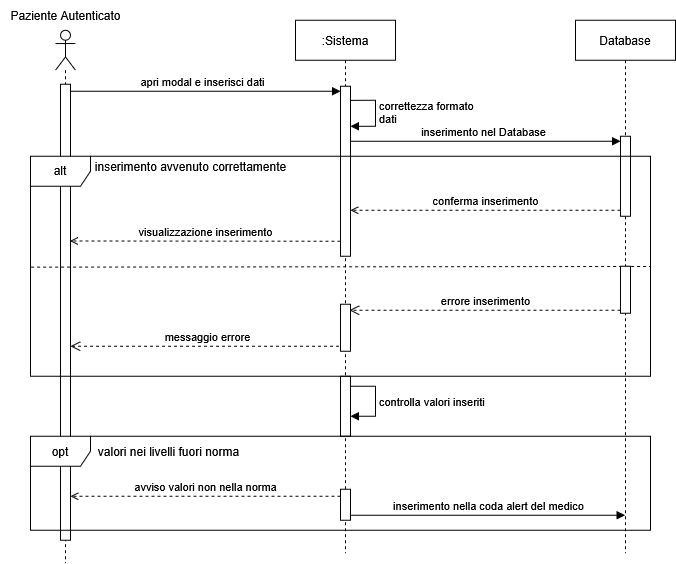
\includegraphics[width=\linewidth, height=0.5\textheight, keepaspectratio]
    {img/Use_case/Inserimento_glicemia.png}
\end{figure}

\subsection{Segnalazione di patologie, malattie e/o sintomi}
Il paziente può segnalare al proprio medico eventuali patologie, malattie e/o
sintomi. Nel riquadro dedicato il paziente può selezionare i vari sintomi dalle
checkbox oppure scriverli liberamente nel campo di testo assieme a eventuali 
malattie e patologie.

\vspace{0.5cm}

\fbox{
    \begin{minipage}{0.9\textwidth}

        \vspace{0.2cm}
        \textbf{Attori: } Paziente \\
        \textbf{Precondizioni: } Il paziente deve essersi autenticato \\
        \textbf{Passi: } \vspace{0.05cm}
        \begin{enumerate}
            \item Il paziente seleziona le checkbox dei sintomi riscontrati
            \item Il paziente compila il campo di testo inserendo patologie e malattie
            \item Il paziente clicca il pulsante "invia segnalazione"
            \item La segnalazione viene comunicata al medico
        \end{enumerate}
        \textbf{Postcondizioni: } La segnalazione viene inserita nel database
        e viene segnalata al medico
    \vspace{0.2cm}
    \end{minipage}
}

\begin{figure}[H]
    \centering
    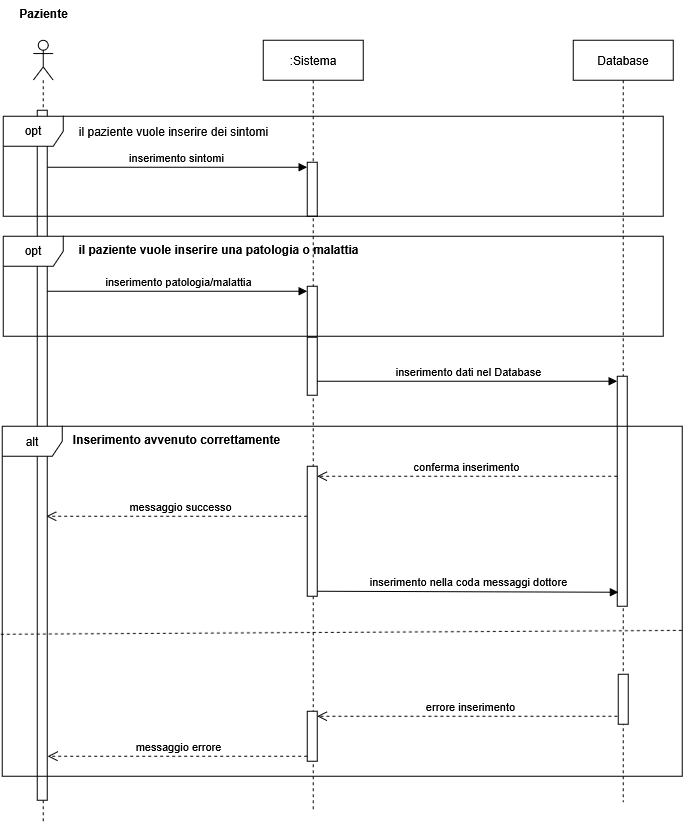
\includegraphics[width=\linewidth, height=0.55\textheight, keepaspectratio]
    {img/Use_case/Segnala_medico.png}
\end{figure}

\vspace{0.5cm}

\subsection{Registrazione giornaliera di medicinali assunti}
Il paziente può registrare i medicinali assunti giornalmente.
Nel riquadro apposito ci sarà la lista dei medicinali che il paziente dovrebbe
assumere durante la giornata, dovrà semplicemente selezionare quelli assunti
e schiacciare il pulsante "invia report al medico" affinchè possano essere registrati.
Inoltre si potrà visualizzare il numero di volte che si è assunto un certo
medicinale in un giorno.

\vspace{0.5cm}

\fbox{
    \begin{minipage}{0.9\textwidth}

        \vspace{0.2cm}
        \textbf{Attori: } Paziente \\
        \textbf{Precondizioni: } Il paziente deve essersi autenticato \\
        \textbf{Passi: } \vspace{0.05cm}
        \begin{enumerate}
            \item Il paziente seleziona i medicinali assunti dalla lista
            \item Il paziente clicca il pulsante "invia report al medico"
            \item Vengono poi controllati i dati inseriti
            \item Infine viene confermata l'avvenuta registrazione dei 
            medicinali o meno
        \end{enumerate}
        \textbf{Postcondizioni: } I medicinali assunti vengono registrati nel
        database
    \vspace{0.2cm}
    \end{minipage}
}

\begin{figure}[H]
    \centering
    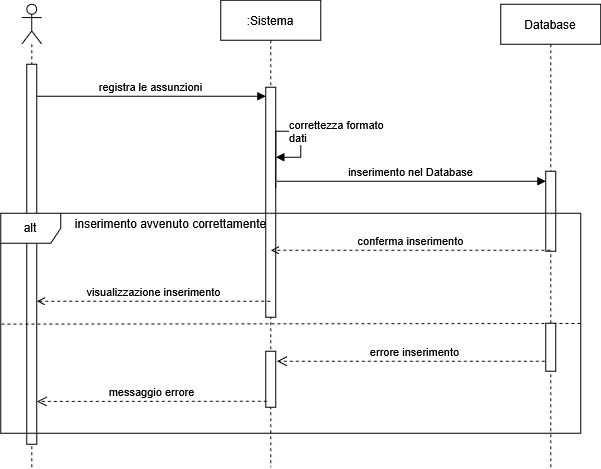
\includegraphics[width=\linewidth, height=0.55\textheight, keepaspectratio]
    {img/Use_case/Medicinali_assunti.png}
\end{figure}

\vspace{0.5cm}

\subsection{Contattare il medico}
Il Paziente può contattare il proprio medico grazie ad un form dedicato.
Nel riquadro apposito il paziente dovrà compilare il campo di testo e selezionare
la priorità del messaggio tra bassa, media e alta; schiacciando poi il tasto
"invia" per inviare il messaggio al medico.

\vspace{0.5cm}

\fbox{
    \begin{minipage}{0.9\textwidth}

        \vspace{0.2cm}
        \textbf{Attori: } Paziente \\
        \textbf{Precondizioni: } Il paziente deve essersi autenticato \\
        \textbf{Passi: } \vspace{0.05cm}
        \begin{enumerate}
            \item Il Paziente compila il campo di testo
            \item Il paziente seleziona la priorità
            \item Il paziente clicca il pulsante "invia"
            \item Viene data conferma dell'avvenuto invio del messaggio o meno 
        \end{enumerate}
        \textbf{Postcondizioni: } Il messaggio viene inviato al medico
    \vspace{0.2cm}
    \end{minipage}
}

\begin{figure}[H]
    \centering
    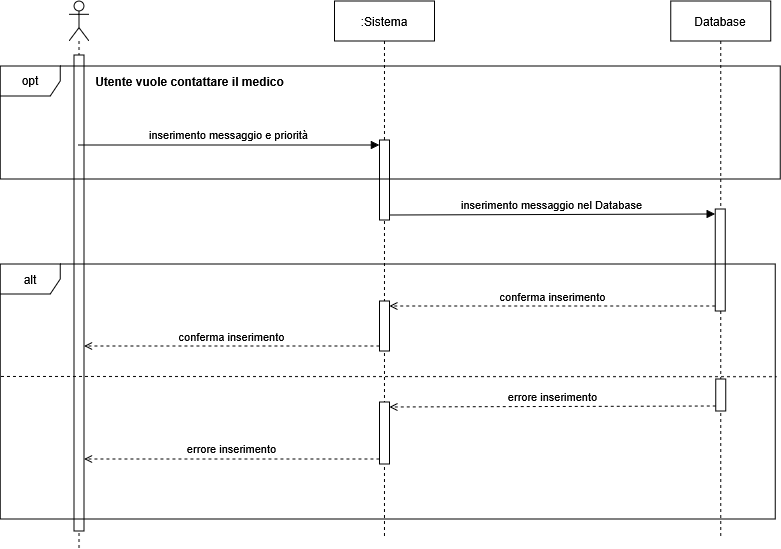
\includegraphics[width=\textwidth, height=\textheight, keepaspectratio]
    {img/Use_case/Contatta_medico.png}
\end{figure}

\section{Casi d'uso del Medico}
\begin{figure}[H]
    \centering
    
\includegraphics[width=\textwidth, height=\textheight, keepaspectratio]
    {img/Use_case/Use_case_medico.png}
\end{figure}

Dopo essersi autenticato il medico verrà reindirizzato alla sua homepage,
dove troverà:
\begin{itemize}
    \item Un riquadro con la lista di messaggi e alert ricevuti
    \item Un'area per la gestione delle terapie dei pazienti
    \item Un'area per la gestione dei pazienti
\end{itemize}

\vspace{1cm}
Ora elenchiamo di seguito i casi d'uso visti nell'immagine:
\begin{itemize}
    \item ricezione e visualizzazione degli alert per il medico
    \item Gestione delle terapie dei pazienti
        \begin{itemize}
            \item Modifica terapia
            \item Elimina terapia
            \item Crea terapia
        \end{itemize}
    \item Gestione dei pazienti
        \begin{itemize}
            \item Visualizza paziente
            \item Modifica paziente
            \item Elimina paziente
        \end{itemize}
\end{itemize}
\vspace{0.5cm}
\subsection{Visualizza alert per il medico}

Il medico avrà la lista dei messaggi e degli alert sulla destra della sua
homepage; quando avrà letto l'alert o non ne necessiterà più potrà schiacciare
il tasto "leggi" per segnarlo come letto e quindi rimuoverlo dalla lista.

\vspace{0.5cm}

\fbox{
    \begin{minipage}{0.9\textwidth}

        \vspace{0.2cm}
        \textbf{Attori: } Medico \\
        \textbf{Precondizioni: } Il medico deve essersi autenticato \\
        \textbf{Passi: } \vspace{0.05cm}
        \begin{enumerate}
            \item Il medico legge l'alert
            \item Il medico clicca il pulsante "leggi" per eliminarlo dalla lista
        \end{enumerate}
        \textbf{Postcondizioni: } l'alert viene rimosso dalla lista del medico
        \vspace{0.2cm}

    \end{minipage}
}

\begin{figure}[H]
    \centering
    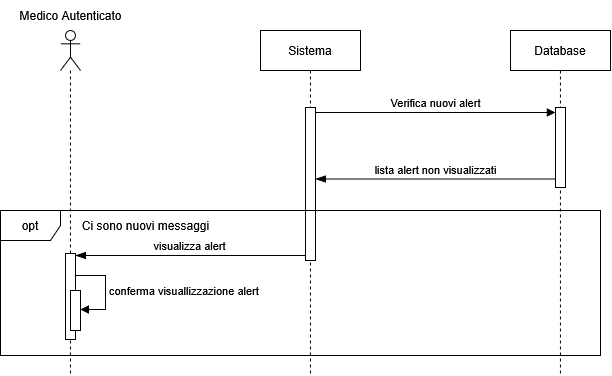
\includegraphics[width=\textwidth, height=\textheight, keepaspectratio]
    {img/Use_case/Vis_alert_medico.png}
\end{figure}

\vspace{0.5cm}


\subsection{Gestione Terapie}
Il medico può decidere di modificare una terapia cliccando il pulsante a forma
di matita affianco alla terapia che vuole modificare; in caso volesse
eliminarla dovrà schiacciare il pulsante a forma di cestino, con conferma dell'eliminazione, 
e infine può decidere di crearne una nuova schiacciando il pulsante "Nuova Terapia".
Nel caso della creazione e della modifica si aprirà un modal nel quale dovrà
inserire i dati richiesti e scegliere il paziente per il quale è stata creata.

\vspace{0.5cm}

\fbox{
    \begin{minipage}{0.9\textwidth}

        \vspace{0.2cm}
        \textbf{Attori: } Medico \\
        \textbf{Precondizioni: } Il medico deve essersi autenticato \\
        \textbf{Passi: } \vspace{0.05cm}
        \begin{enumerate}
            \item Modifica terapia
            \begin{enumerate}
                \item Il medico schiaccia il pulsante a forma di matita
                \item Il medico modifica i dati del modal della terapia
                \item Il medico schiaccia il pulsante "salva"
            \end{enumerate}
            \item Aggiungi terapia
            \begin{enumerate}
                \item Il medico schiaccia il pulsante "Nuova Terapia"
                \item Il medico compila i campi richiesti nel modal
                \item Il medico schiaccia il pulsante "salva"
            \end{enumerate}
            \item Elimina terapia
            \begin{enumerate}
                \item Il medico schiaccia il pulsante a forma di cestino affianco
                alla terapia che desidera eliminare
                \item Il medico conferma l'eliminazione della terapia
            \end{enumerate}
        \end{enumerate}
        \textbf{Postcondizioni: } La terapia viene modificata, creata o eliminata
        in base alle decisioni del medico
        \vspace{0.2cm}

    \end{minipage}
}

\begin{figure}[H]
    \centering
    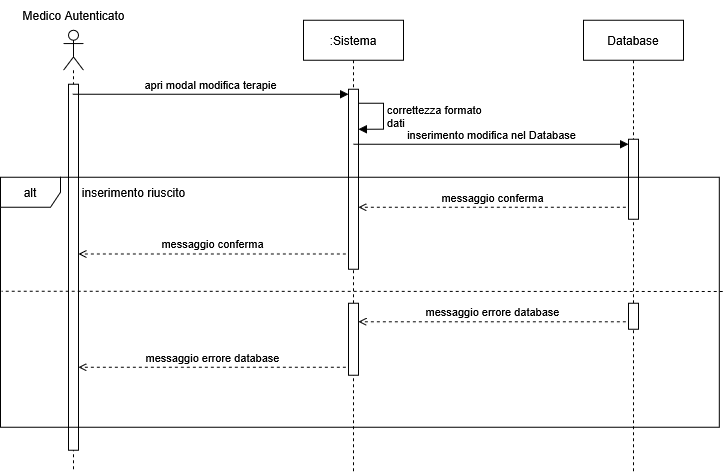
\includegraphics[width=\linewidth, height=\textheight, keepaspectratio]
    {img/Use_case/Modifica_terapie.png}
    \caption{Modifica Terapia}
\end{figure}

\begin{figure}[H]
    \centering
    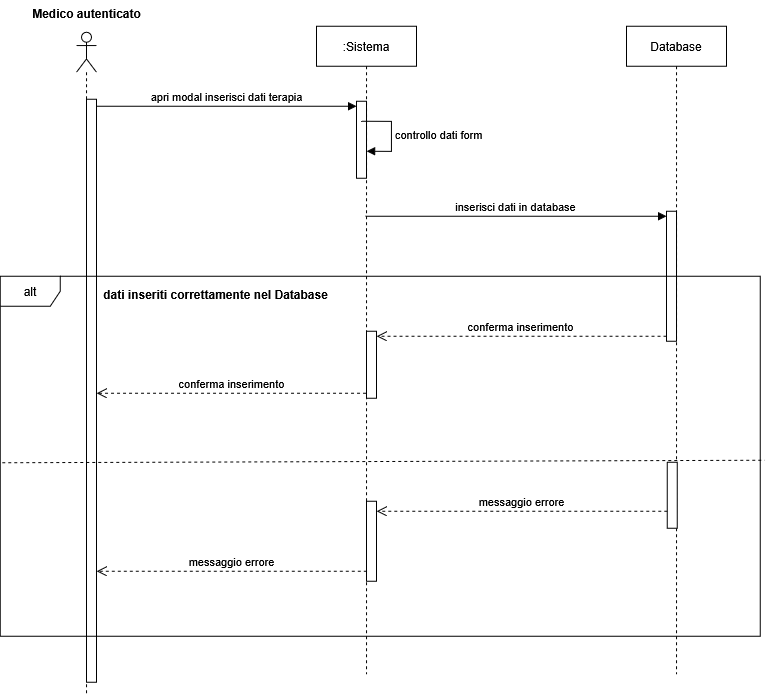
\includegraphics[width=\linewidth, height=\textheight, keepaspectratio]
    {img/Use_case/Crea_terapie.png}
    \caption{Crea Terapia}
\end{figure}

\begin{figure}[H]
    \centering
    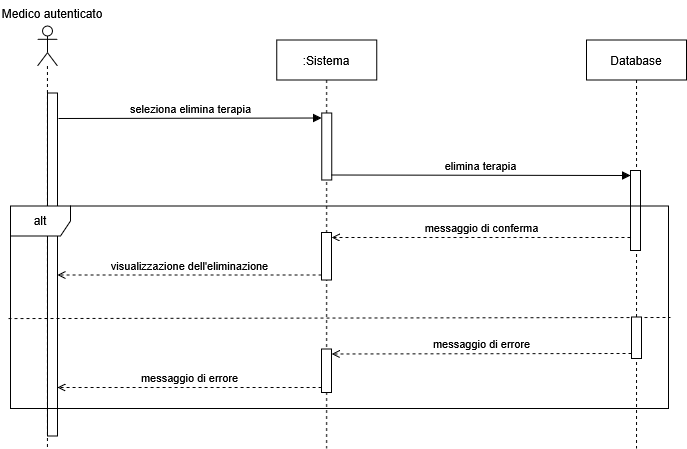
\includegraphics[width=\linewidth, height=\textheight, keepaspectratio]
    {img/Use_case/Elimina_terapie.png}
    \caption{Elimina Terapia}
\end{figure}
\newpage
\subsection{Gestione Pazienti}
Il medico può decidere di modificare le informazioni di un Paziente cliccando il
pulsante a forma di matita affianco al paziente del quale vuole modificare i dati;
in caso volesse eliminarlo dovrà schiacciare il pulsante a forma di cestino;
nel caso voglia solo visualizzare l'andamento glicemico bisogna che schiacci il 
pulsante a forma di occhio.
Nel caso della creazione si aprirà un modal nel quale dovrà
inserire i dati richiesti e scegliere il paziente per il quale è stata creata.


\vspace{0.5cm}

\fbox{
    \begin{minipage}{0.9\textwidth}

        \vspace{0.2cm}
        \textbf{Attori: } Medico \\
        \textbf{Precondizioni: } Il medico deve essersi autenticato \\
        \textbf{Passi: } \vspace{0.05cm}
        \begin{enumerate}
            \item Modifica dati del Paziente
            \begin{enumerate}
                \item Il medico schiaccia il pulsante a forma di matita
                \item Il medico modifica i dati del modal del paziente
                \item Il medico schiaccia il pulsante "salva"
            \end{enumerate}
            \item Visualizza dati Paziente
            \begin{enumerate}
                \item Il medico schiaccia il pulsante a forma di occhio
            \end{enumerate}
            \item Elimina Paziente
            \begin{enumerate}
                \item Il medico schiaccia il pulsante a forma di cestino affianco
                al paziente che desidera eliminare
                \item Il medico conferma l'eliminazione del paziente
            \end{enumerate}
        \end{enumerate}
        \textbf{Postcondizioni: } Il paziente viene modificato o eliminato
        in base alle decisioni del medico, oppure vengono visualizzati i suoi dati
        \vspace{0.2cm}

    \end{minipage}
}

\begin{figure}[H]
    \centering
    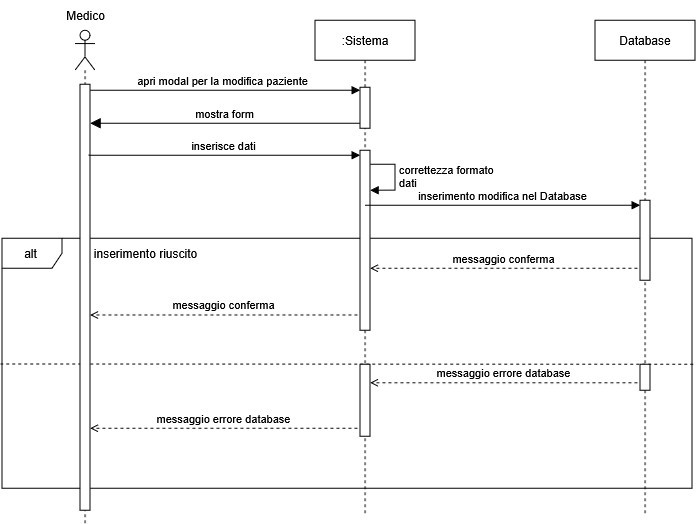
\includegraphics[width=\textwidth, height=0.5\textheight, keepaspectratio]
    {img/Use_case/Modifica_paziente.png}
    \caption{Modifica Paziente}
\end{figure}

\begin{figure}[H]
    \centering
    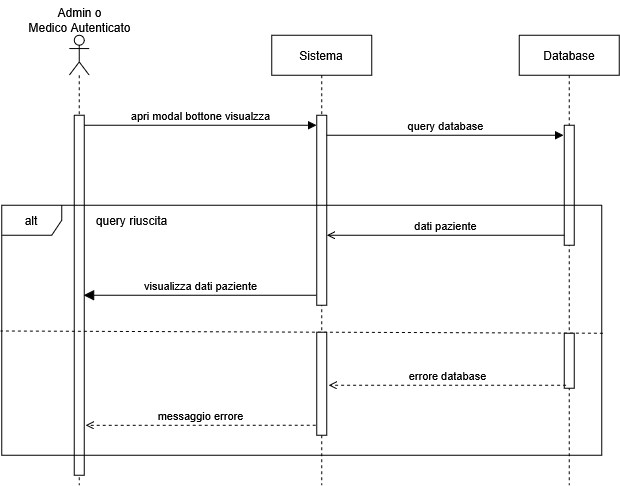
\includegraphics[width=\textwidth, height=\textheight, keepaspectratio]
    {img/Use_case/Visualizza_paziente.png}
    \caption{Visualizza Paziente}
\end{figure}

\begin{figure}[H]
    \centering
    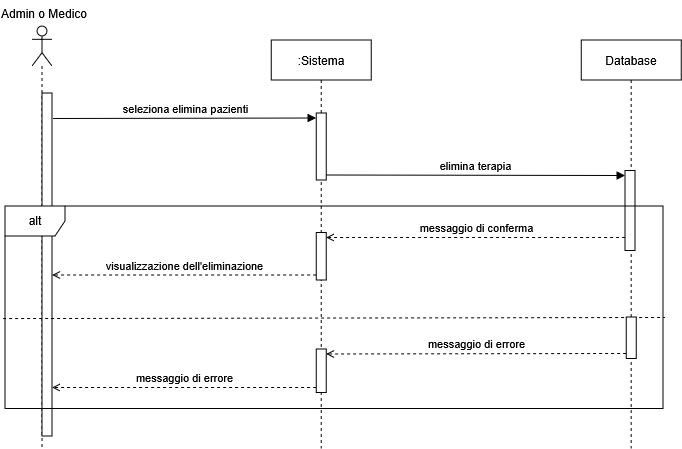
\includegraphics[width=\textwidth, height=\textheight, keepaspectratio]
    {img/Use_case/Elimina_pazienti.png}
    \caption{Elimina Paziente}
\end{figure}

\section{Casi d'uso dell'Admin}
\begin{figure}[H]
    \centering
    
\includegraphics[width=\textwidth, height=\textheight, keepaspectratio]
    {img/Use_case/Use_case_admin.png}
\end{figure}

Dopo essersi autenticato l'admin verrà reindirizzato alla sua homepage,
dove troverà:
\begin{itemize}
    \item Gestione utenti
    \begin{itemize}
        \item Gestisci Pazienti
        \item Gestisci Medici
    \end{itemize}
    \item Lista dei log del sistema
\end{itemize}

\newpage

\vspace{1cm}
Ora elenchiamo di seguito i casi d'uso visti nell'immagine:
\begin{itemize}
    \item Visualizzazione dei log di sistema
    \item Gestione dei Pazienti
    \begin{itemize}
        \item Visualizza paziente
        \item Modifica paziente
        \item Elimina paziente
        \item Crea paziente
    \end{itemize}
    \item Gestione dei Medici
    \begin{itemize}
        \item Modifica medico
        \item Elimina medico
        \item Crea medico
    \end{itemize}
\end{itemize}
\vspace{0.5cm}
\subsection{Visualizza log}
L'admin può visualizzare i log del sistema per monitorare le attività compiute
dagli utenti.

\vspace{0.5cm}

\fbox{
    \begin{minipage}{0.9\textwidth}

        \vspace{0.2cm}
        \textbf{Attori: } Admin \\
        \textbf{Precondizioni: } l'Admin deve essersi autenticato \\
        \textbf{Passi: } \vspace{0.05cm}
        \begin{enumerate}
            \item visualizza i log del sistema
        \end{enumerate}
        \vspace{0.2cm}

    \end{minipage}
}
\newpage
\subsection{Gestisci Pazienti}
L'admin può gestire i pazienti al posto del dottore in caso di necessità
come il dottore può modificare, creare, eliminare e visualizzare i pazienti.

\vspace{0.5cm}

\fbox{
    \begin{minipage}{0.9\textwidth}

        \vspace{0.2cm}
        \textbf{Attori: } Admin \\
        \textbf{Precondizioni: } l'Admin deve essersi autenticato \\
        \textbf{Passi: } \vspace{0.05cm}
        \begin{enumerate}
            \item Modifica Paziente
            \begin{enumerate}
                \item L'Admin schiaccia il pulsante a forma di matita
                \item L'Admin modifica i dati del modal del paziente
                \item L'Admin schiaccia il pulsante "salva"
            \end{enumerate}
            \item Visualizza Paziente
            \begin{enumerate}
                \item L'Admin schiaccia il pulsante a forma di occhio
            \end{enumerate}
            \item Elimina Paziente
            \begin{enumerate}
                \item L'Admin schiaccia il pulsante a forma di cestino affianco
                al paziente che desidera eliminare
                \item L'Admin coferma l'eliminazione del paziente
            \end{enumerate}
            \item Crea Paziente
            \begin{enumerate}
                \item l'Admin schiaccia il pulsante "Nuovo Paziente"
                \item L'Admin compila i campi richiesti nel modal
                \item L'admin schiaccia il pulsante "Registra"
            \end{enumerate}
        \end{enumerate}
        \textbf{Postcondizioni: } Il paziente viene modificato, eliminato o creato
        in base alle decisioni dell'Admin, oppure vengono visualizzati i dati del
        paziente.
        \vspace{0.2cm}

    \end{minipage}
}

\begin{figure}[H]
    \centering
    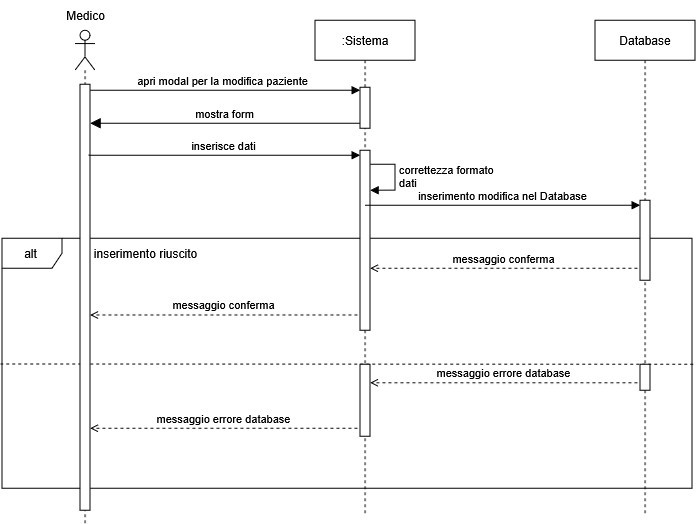
\includegraphics[width=\textwidth, height=\textheight, keepaspectratio]
    {img/Use_case/Modifica_paziente.png}
    \caption{Modifica Paziente}
\end{figure}

\begin{figure}[H]
    \centering
    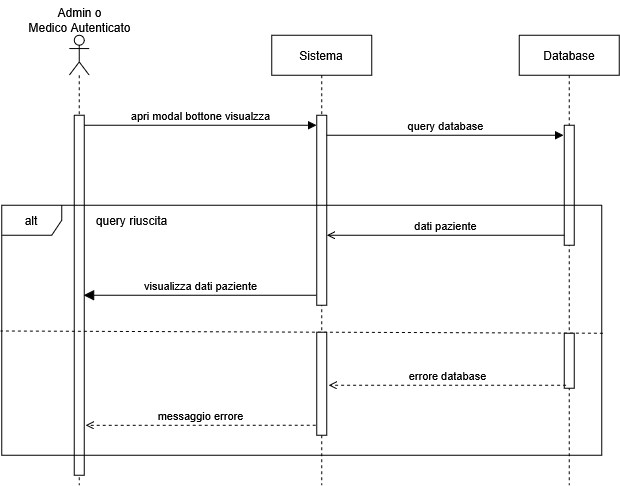
\includegraphics[width=\textwidth, height=\textheight, keepaspectratio]
    {img/Use_case/Visualizza_paziente.png}
    \caption{Visualizza Paziente}
\end{figure}

\begin{figure}[H]
    \centering
    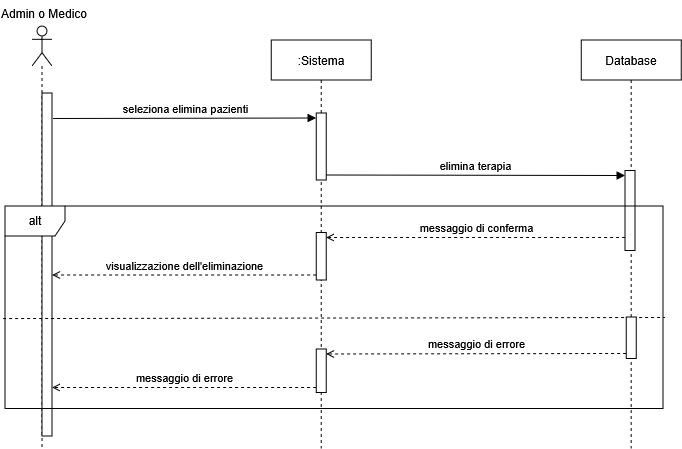
\includegraphics[width=\textwidth, height=\textheight, keepaspectratio]
    {img/Use_case/Elimina_pazienti.png}
    \caption{Elimina Paziente}
\end{figure}

\begin{figure}[H]
    \centering
    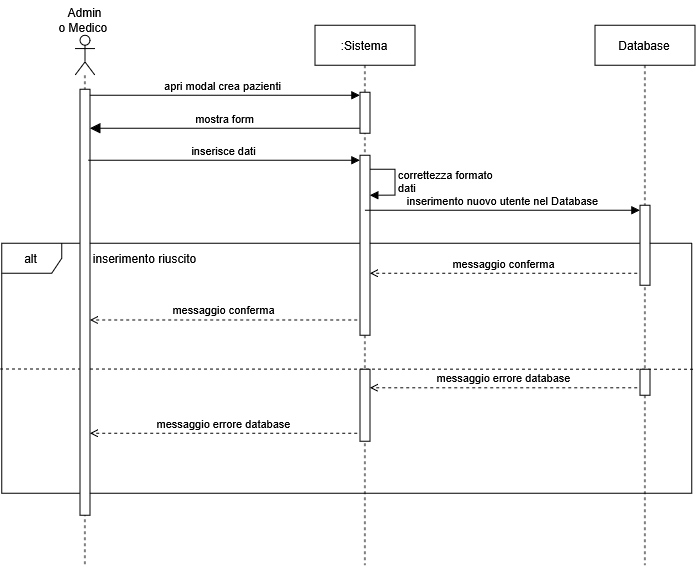
\includegraphics[width=\textwidth, height=\textheight, keepaspectratio]
    {img/Use_case/Crea_paziente.png}
    \caption{Crea Paziente}
\end{figure}
\newpage
\subsection{Gestisci Medici}
L'Admin può decidere di modificare le informazioni di un medico cliccando il
pulsante a forma di matita affianco al medico del quale vuole modificare i dati;
in caso volesse eliminarlo dovrà schiacciare il pulsante a forma di cestino;
Nel caso della creazione si aprirà un modal nel quale dovrà inserire i dati richiesti.

\vspace{0.5cm}

\fbox{
    \begin{minipage}{0.9\textwidth}

        \vspace{0.2cm}
        \textbf{Attori: } Medico \\
        \textbf{Precondizioni: } Il medico deve essersi autenticato \\
        \textbf{Passi: } \vspace{0.05cm}
        \begin{enumerate}
            \item Modifica Medico
            \begin{enumerate}
                \item L'Admin schiaccia il pulsante a forma di matita
                \item L'Admin modifica i dati del modal del medico
                \item L'Admin schiaccia il pulsante "salva"
            \end{enumerate}
            \item Elimina Medico
            \begin{enumerate}
                \item L'Admin schiaccia il pulsante a forma di cestino affianco
                al medico che desidera eliminare
                \item L'Admin conferma l'eliminazione del medico
            \end{enumerate}
            \item Crea Medico
            \begin{enumerate}
                \item l'Admin schiaccia il pulsante "Nuovo Medico"
                \item L'Admin compila i campi richiesti nel modal
                \item L'admin schiaccia il pulsante "Registra"
            \end{enumerate}
        \end{enumerate}
        \textbf{Postcondizioni: } Il Medico viene modificato, eliminato o creato
        in base alle decisioni dell'Admin.
        \vspace{0.2cm}

    \end{minipage}
}

\begin{figure}[H]
    \centering
    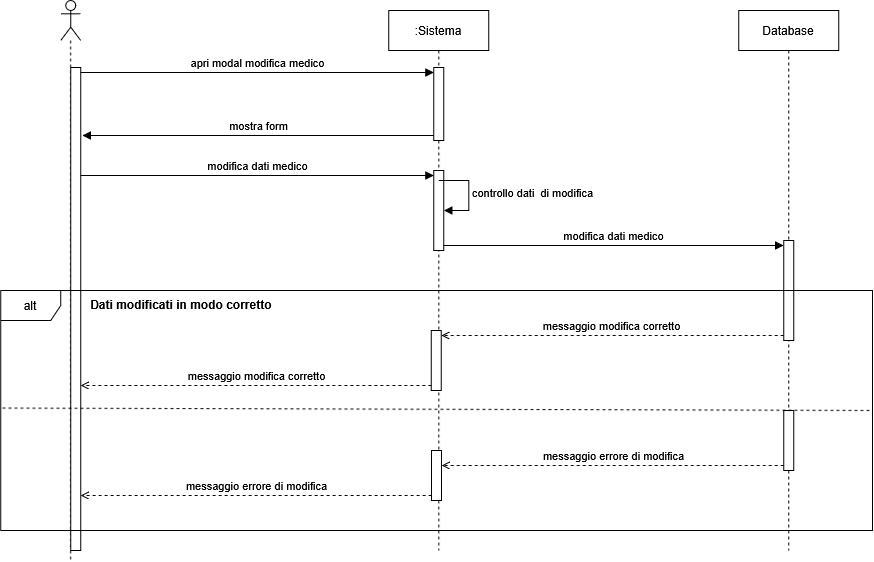
\includegraphics[width=\textwidth, height=\textheight, keepaspectratio]
    {img/Use_case/Modifica_medico.png}
    \caption{Modifica Medico}
\end{figure}

\begin{figure}[H]
    \centering
    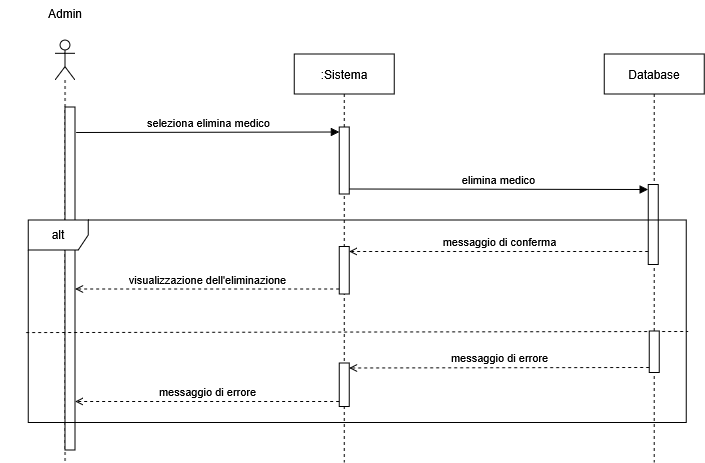
\includegraphics[width=\textwidth, height=\textheight, keepaspectratio]
    {img/Use_case/Elimina_medico.png}
    \caption{Elimina Medico}
\end{figure}

\begin{figure}[H]
    \centering
    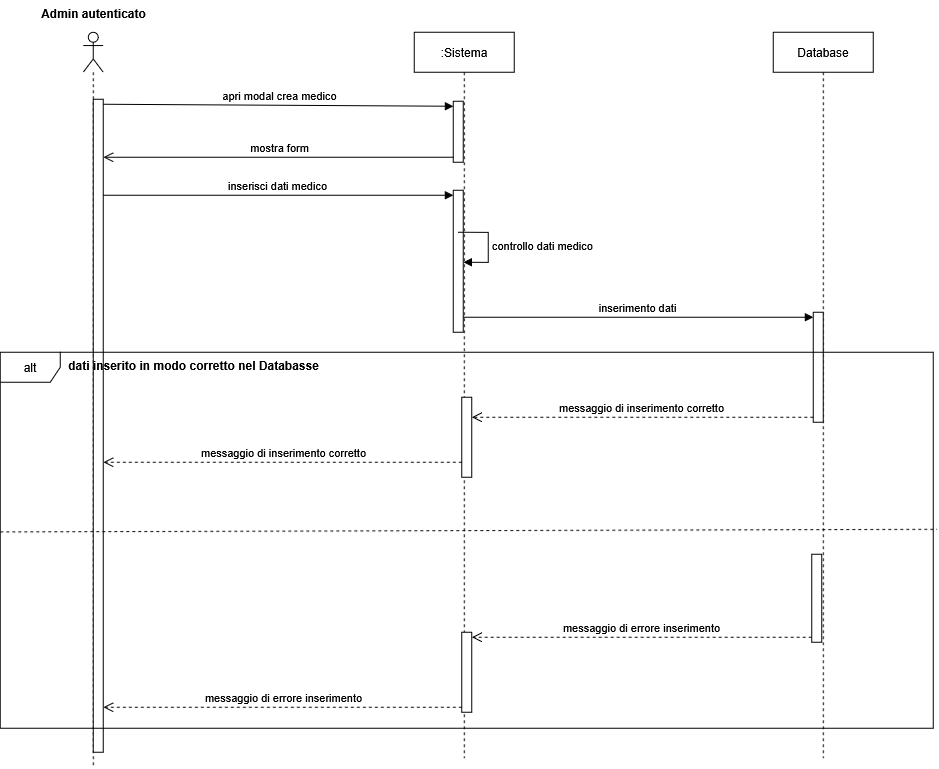
\includegraphics[width=\textwidth, height=\textheight, keepaspectratio]
    {img/Use_case/Crea_medico.png}
    \caption{Crea Medico}
\end{figure}

\chapter{Diagrammi di attività}
Andiamo di seguito a mostrare i diagrammi di attività di ciascuna tipologia
di utente.


\section{Diagramma di autenticazione}

\begin{figure}[H]
    \centering
    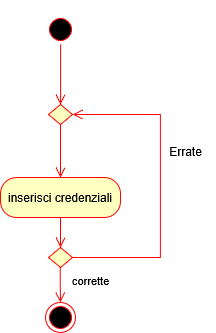
\includegraphics[width=\textwidth, height=0.5\textheight, keepaspectratio]
    {img/Diagrammi/DA_autenticazione.png}
    \caption{Diagramma dell'autenticazione di un utente}
\end{figure}

Per i successivi diagrammi di attività presupponiamo che l'utente abbia già
effettuato l'autenticazione.
I diagrammi verranno visualizzati prima completi con per ogni utente e poi
divisi per avere una più nitida visualizzazione delle varie sezioni.
Le immagini delle diverse sezioni possono avere una struttura diversa da quella
nella foto principale a causa del ridimensionamento per una migliore
visualizzazione.

\section{Diagramma del paziente}

\begin{figure}[H]
    \centering
    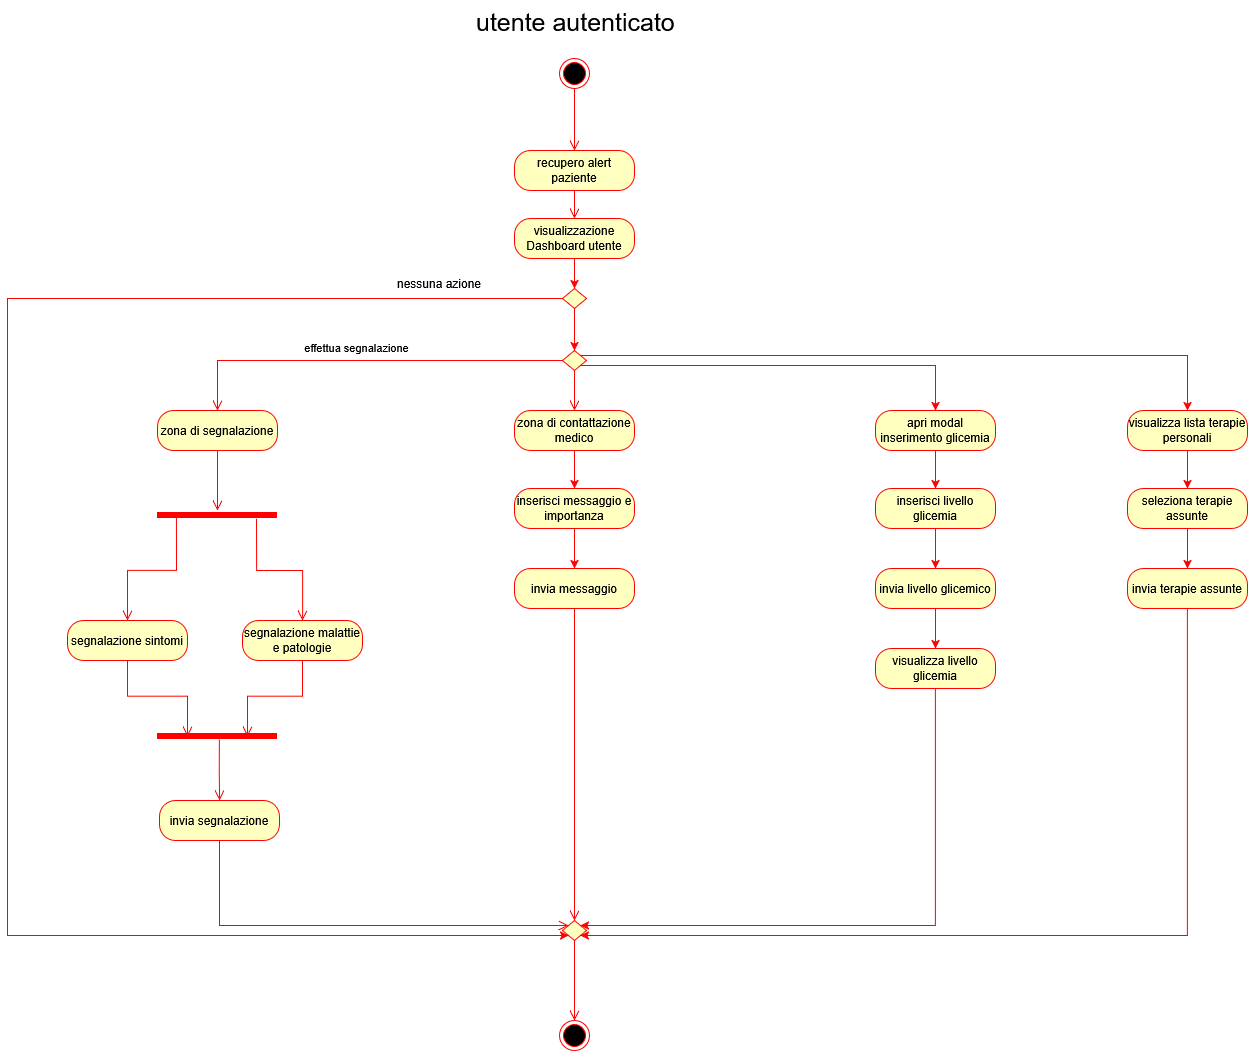
\includegraphics[width=\textwidth, height=\textheight, keepaspectratio]
    {img/Diagrammi/DA_paziente.png}
\end{figure}

\subsection{Diagramma per la segnalazione di patologie, malattie e/o sintomi}
\begin{figure}[H]
    \centering
    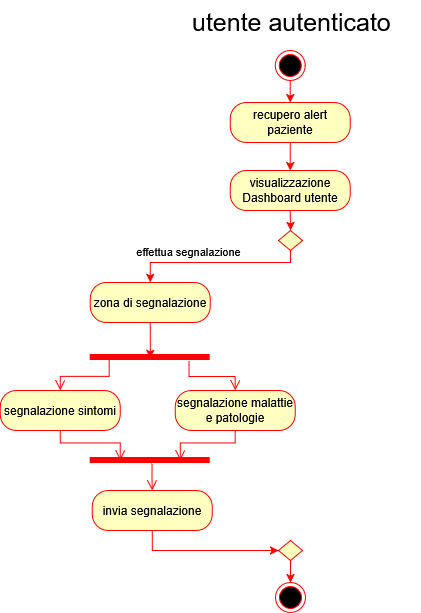
\includegraphics[width=\textwidth, height=0.9\textheight, keepaspectratio]
    {img/Diagrammi/DA_paziente_0.png}
\end{figure}

\subsection{Diagramma di come un paziente comunica con il medico}
\begin{figure}[H]
    \centering
    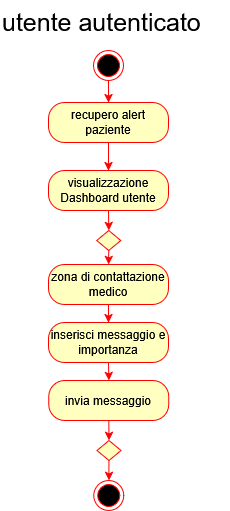
\includegraphics[width=\textwidth, height=0.9\textheight, keepaspectratio]
    {img/Diagrammi/DA_paziente_1.png}
\end{figure}

\subsection{Diagramma per l'inserimento della glicemia}
\begin{figure}[H]
    \centering
    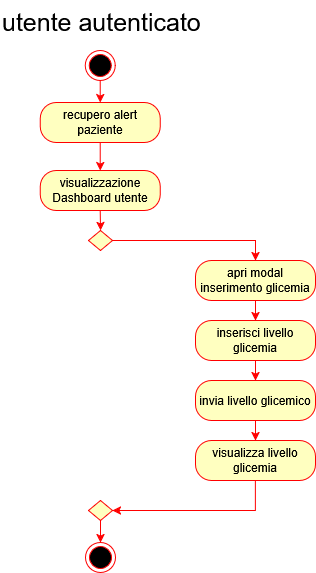
\includegraphics[width=\textwidth, height=0.9\textheight, keepaspectratio]
    {img/Diagrammi/DA_paziente_2.png}
\end{figure}

\subsection{Diagramma per la registrazione giornaliera dei medicinali}
\begin{figure}[H]
    \centering
    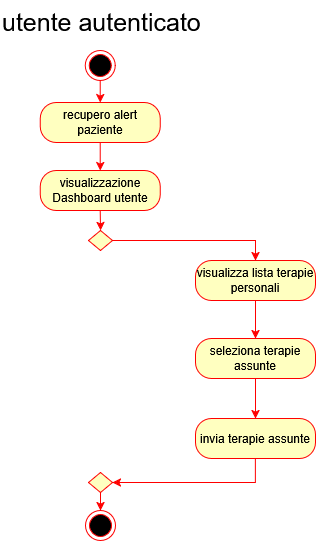
\includegraphics[width=\textwidth, height=0.9\textheight, keepaspectratio]
    {img/Diagrammi/DA_paziente_3.png}
\end{figure}



\section{Diagramma del medico}

\begin{figure}[H]
    \centering
    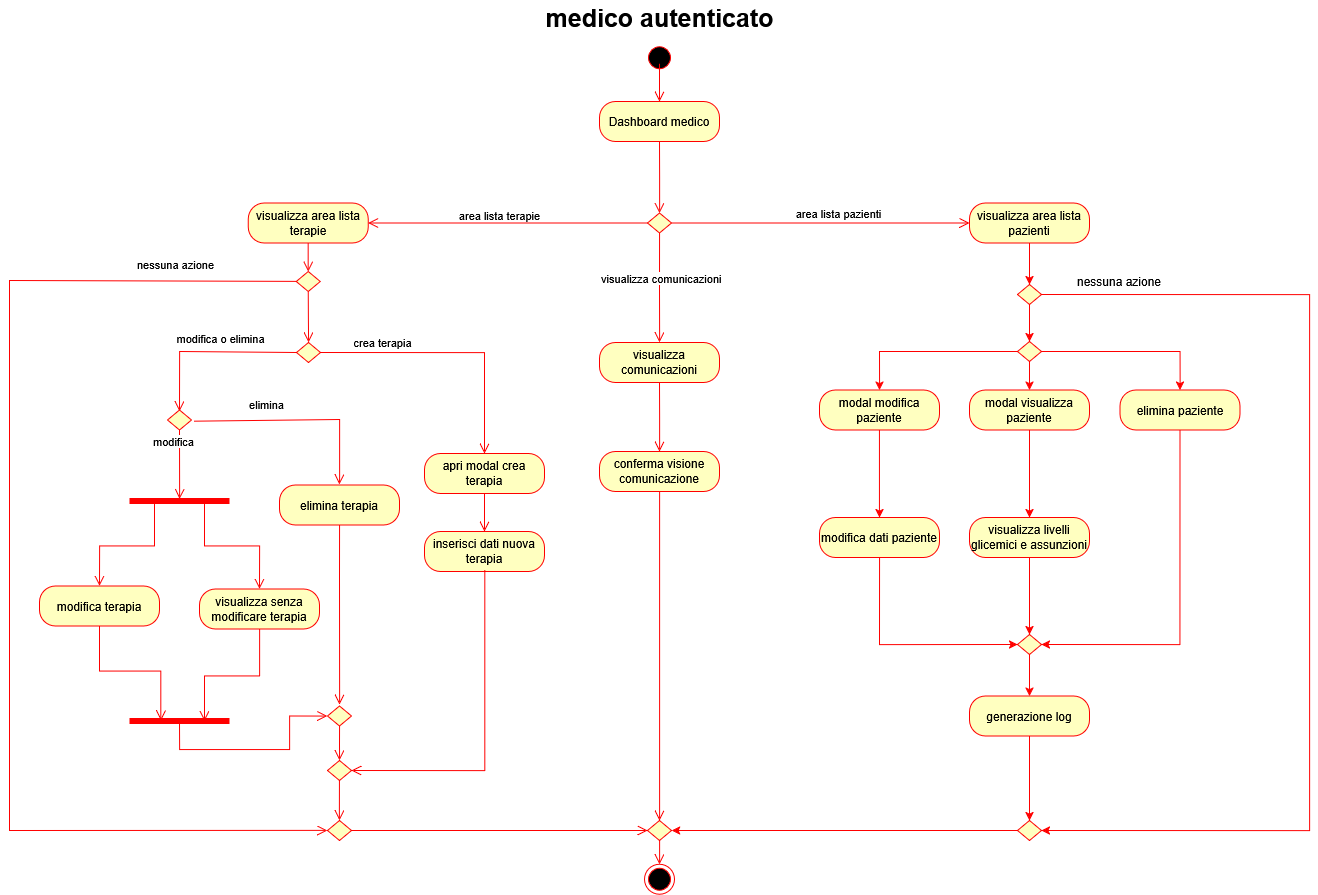
\includegraphics[width=\textwidth, height=\textheight, keepaspectratio]
    {img/Diagrammi/DA_medico.png}
    \caption{Diagramma completo del medico}
\end{figure}


\subsection{Diagramma di gestione delle terapie}
\begin{figure}[H]
    \centering
    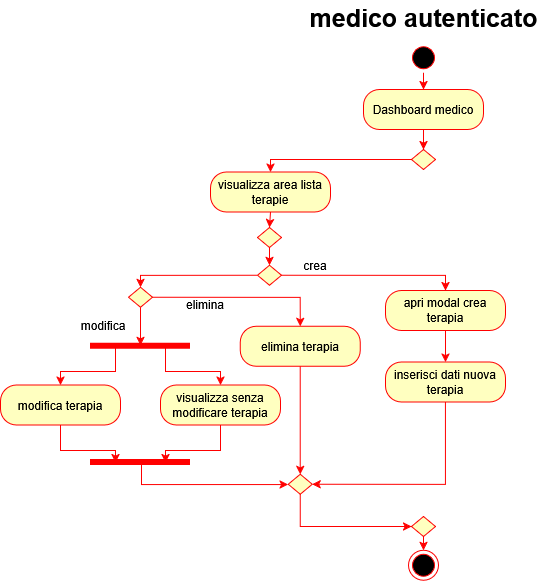
\includegraphics[width=\textwidth, height=0.9\textheight, keepaspectratio]
    {img/Diagrammi/DA_medico_0.png}
\end{figure}

\subsection{Diagramma di visualizzazione degli alert del medico}
\begin{figure}[H]
    \centering
    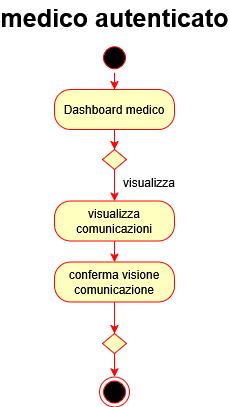
\includegraphics[width=\textwidth, height=0.9\textheight, keepaspectratio]
    {img/Diagrammi/DA_medico_1.png}
\end{figure}

\subsection{Diagramma di gestione dei pazienti}
\begin{figure}[H]
    \centering
    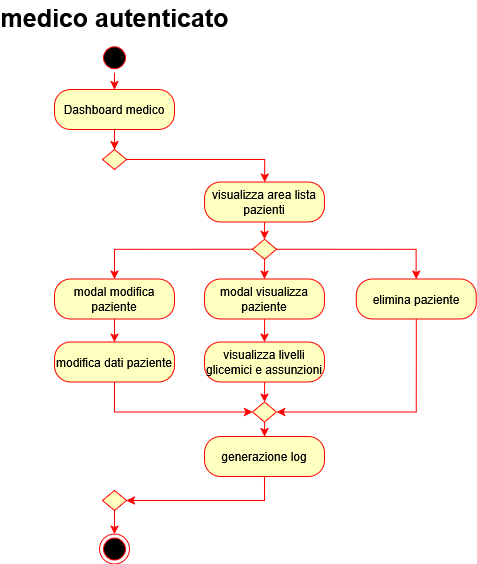
\includegraphics[width=\textwidth, height=0.9\textheight, keepaspectratio]
    {img/Diagrammi/DA_medico_2.png}
\end{figure}

\section{Diagramma dell'admin}

\begin{figure}[H]
    \centering
    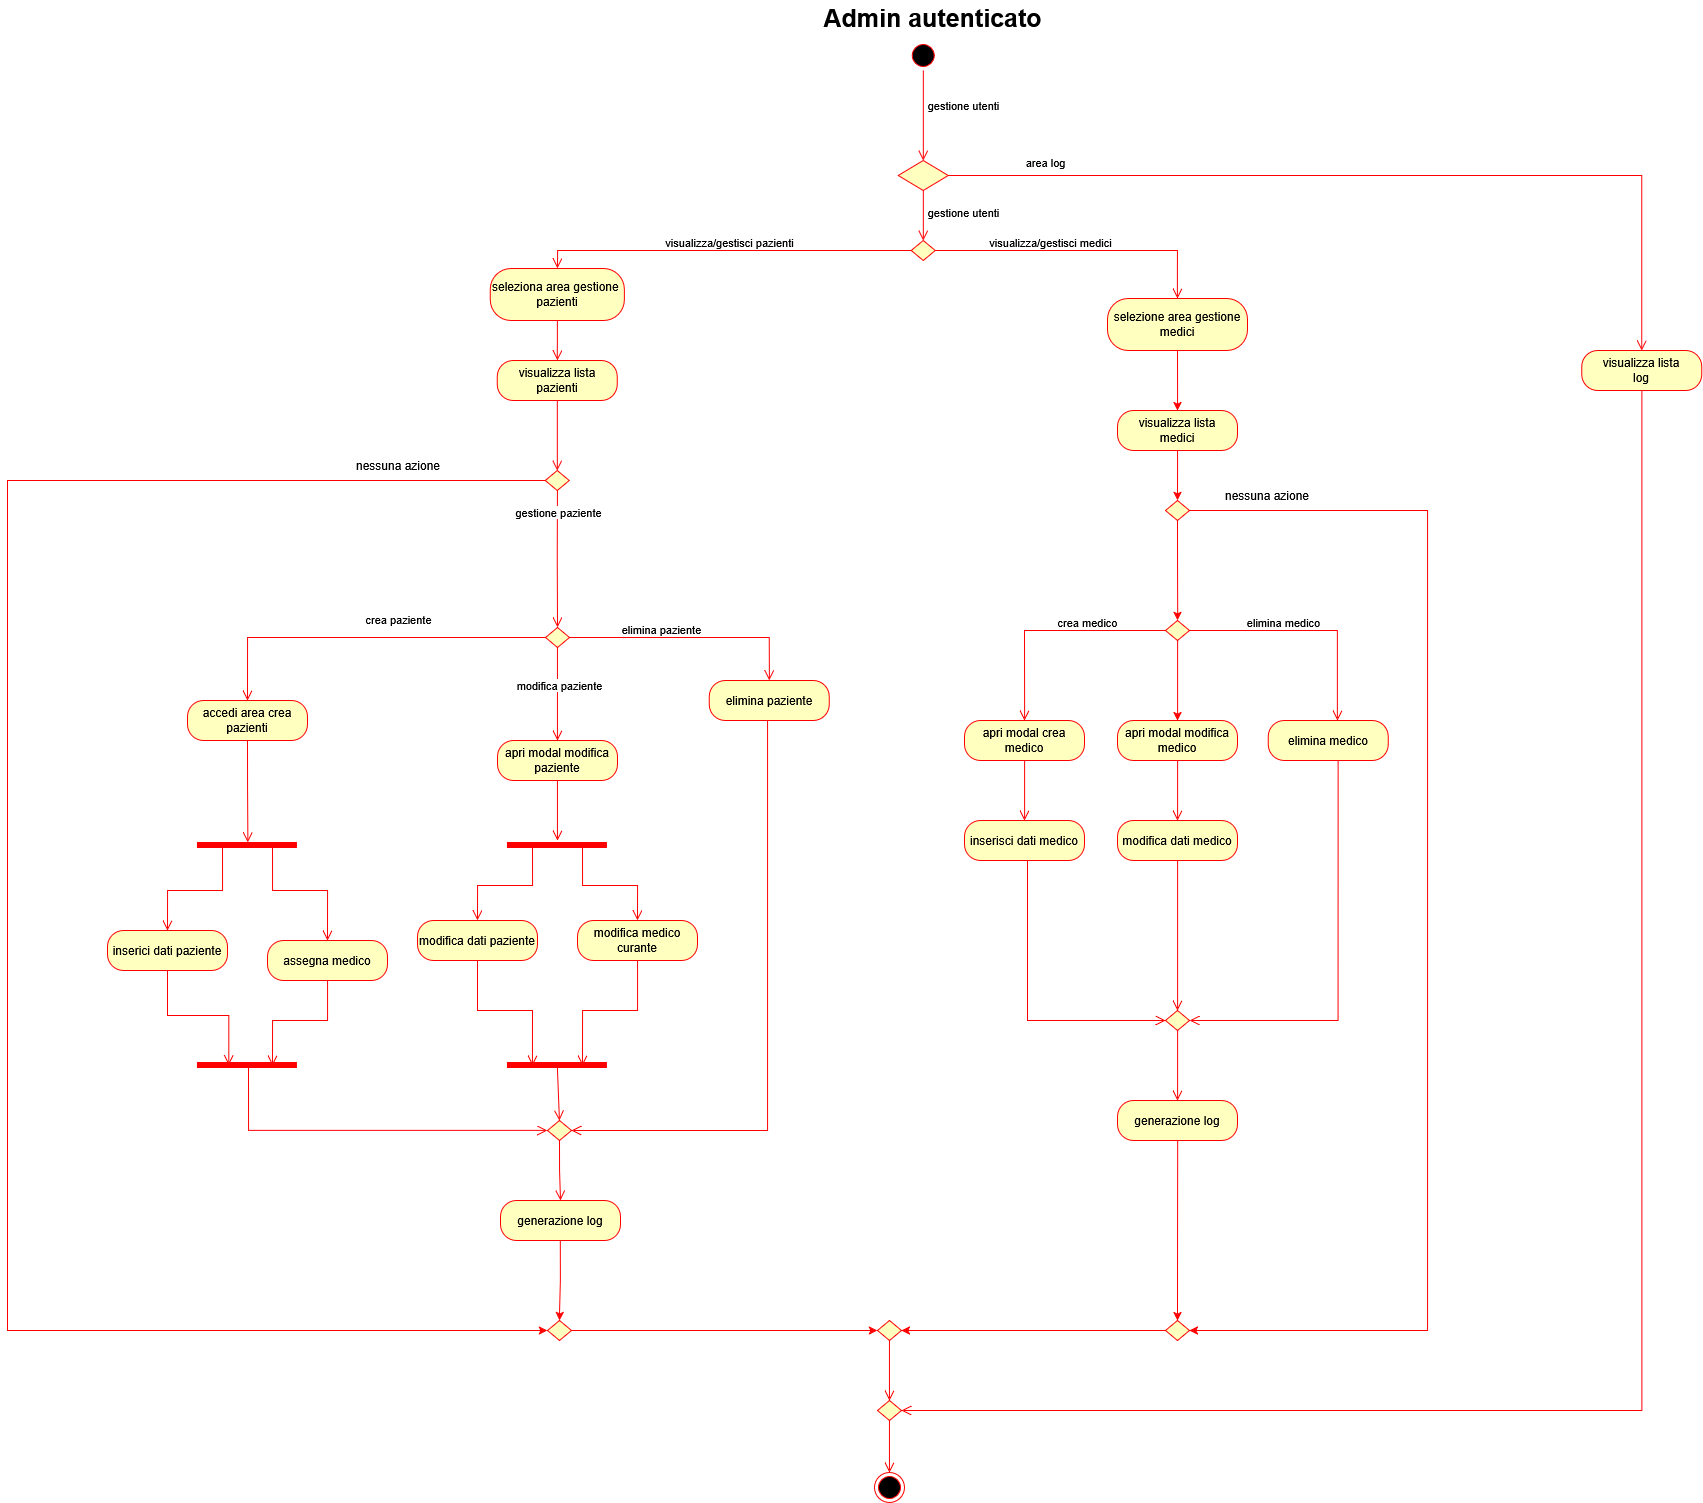
\includegraphics[width=\textwidth, height=\textheight, keepaspectratio]
    {img/Diagrammi/DA_admin.png}
    \caption{Diagramma completo dell'admin}
\end{figure}

\subsection{Diagramma gestione dei pazienti}
\begin{figure}[H]
    \centering
    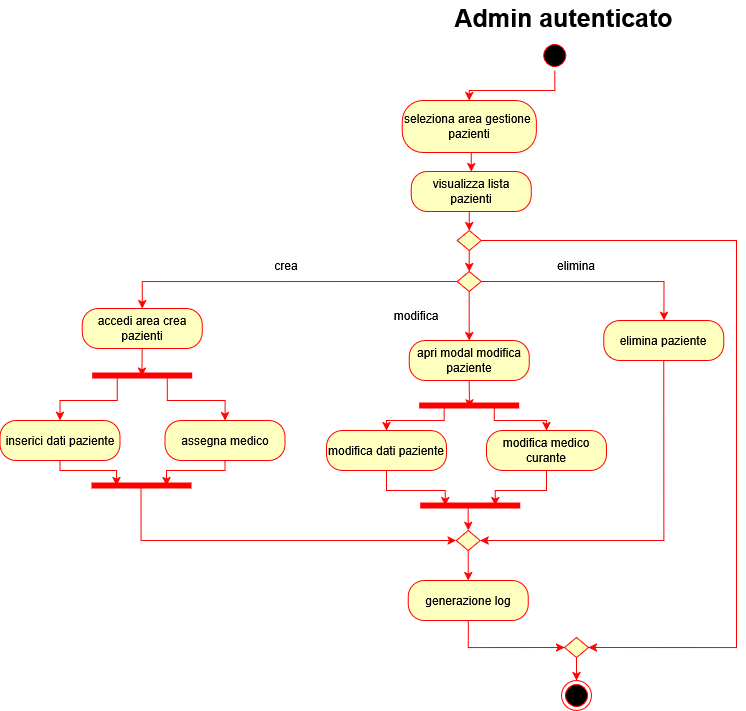
\includegraphics[width=\textwidth, height=0.9\textheight, keepaspectratio]
    {img/Diagrammi/DA_admin_0.png}
\end{figure}

\subsection{Diagramma della gestione dei medici}
\begin{figure}[H]
    \centering
    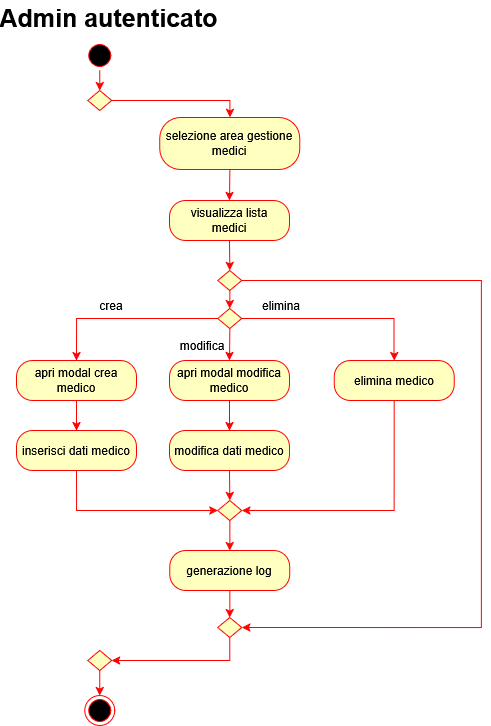
\includegraphics[width=\textwidth, height=0.9\textheight, keepaspectratio]
    {img/Diagrammi/DA_admin_1.png}
\end{figure}

\subsection{Diagramma visualizzazione dei log}
\begin{figure}[H]
    \centering
    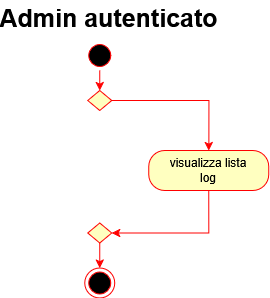
\includegraphics[width=\textwidth, height=0.9\textheight, keepaspectratio]
    {img/Diagrammi/DA_admin_2.png}
\end{figure}



\chapter{Diagrammi UML}

\section{Diagramma delle classi - Package Entity}

Il package \texttt{entity} definisce la rappresentazione a oggetti dello schema dati. Di seguito è mostrato il diagramma UML delle entità JPA, che costituiscono il nucleo del sistema, con particolare enfasi sulla mappatura delle relazioni e sulla definizione degli attributi.
\begin{figure}[H]
    \centering
    
\includegraphics[width=0.98\textwidth, keepaspectratio]
    {img/UML/entity_class_diagram.png}
    \caption{Diagramma delle classi - Package Entity}
    \label{fig:class_diagram_entity}
\end{figure}

\subsection{Entità principali}

\textbf{Utente:}
\begin{itemize}
    \item Classe base per tutti gli utenti del sistema
    \item Utilizza strategia di ereditarietà JOINED (tabelle separate per sottoclassi)
    \item Contiene dati anagrafici comuni: email, password, nome, cognome, data nascita
    \item Campo \texttt{ruolo} per distinguere: ROLE\_PAZIENTE, ROLE\_MEDICO, ROLE\_ADMIN
\end{itemize}

\textbf{Paziente} (estende Utente):
\begin{itemize}
    \item Aggiunge informazioni cliniche: fattoriRischio, comorbita, patologiePregresse
    \item Associato a un medico curante (relazione ManyToOne con Utente)
    \item Possiede collezioni di: Rilevazione, Comunicazione, Terapia, Assunzione
\end{itemize}

\textbf{Terapia:}
\begin{itemize}
    \item Rappresenta una prescrizione farmacologica
    \item Attributi: farmaco, numAssunzioni, dosaggio, indicazioni
    \item Prescritta da un medico (ManyToOne con Utente)
    \item Associata a un paziente (ManyToOne con Paziente)
    \item Genera assunzioni registrate dal paziente (OneToMany con Assunzione)
\end{itemize}

\textbf{Assunzione:}
\begin{itemize}
    \item Registra quando il paziente assume un farmaco
    \item Associata a una Terapia specifica (ManyToOne)
    \item Include timestamp per tracciamento temporale
\end{itemize}

\textbf{Rilevazione:}
\begin{itemize}
    \item Memorizza una misurazione della glicemia
    \item Attributi: valore (Double in mg/dL), timestamp
    \item Associata a un paziente (ManyToOne)
    \item Range normale: 80-130 mg/dL (80-180 mg/dL dopo i pasti)
\end{itemize}

\textbf{Comunicazione:}
\begin{itemize}
    \item Messaggi e alert tra paziente e medico
    \item Livello di priorità: 1=bassa, 2=media, 3=alta
    \item Flag \texttt{letto} per gestire stato lettura
    \item Può essere generata automaticamente dal sistema (alert)
\end{itemize}

\textbf{Log:}
\begin{itemize}
    \item Registro eventi di sistema per audit
    \item Attributi: tipo, descrizione, timestamp
    \item Entità standalone senza relazioni
\end{itemize}

\textbf{BlacklistedToken:}
\begin{itemize}
    \item Gestione token JWT invalidati (logout)
    \item Chiave primaria: jti (JWT ID univoco)
    \item Include expiry per cleanup automatico token scaduti
\end{itemize}

%------------------------------------------------------------------------------
\section{Diagrammi di sequenza UML}

%..............................................................................
\subsection{Autenticazione (Sign-In)}

Il processo di autenticazione permette agli utenti di accedere al sistema
utilizzando email e password. L'autenticazione è gestita tramite JWT (JSON Web Token).

\begin{figure}[H]
    \centering
    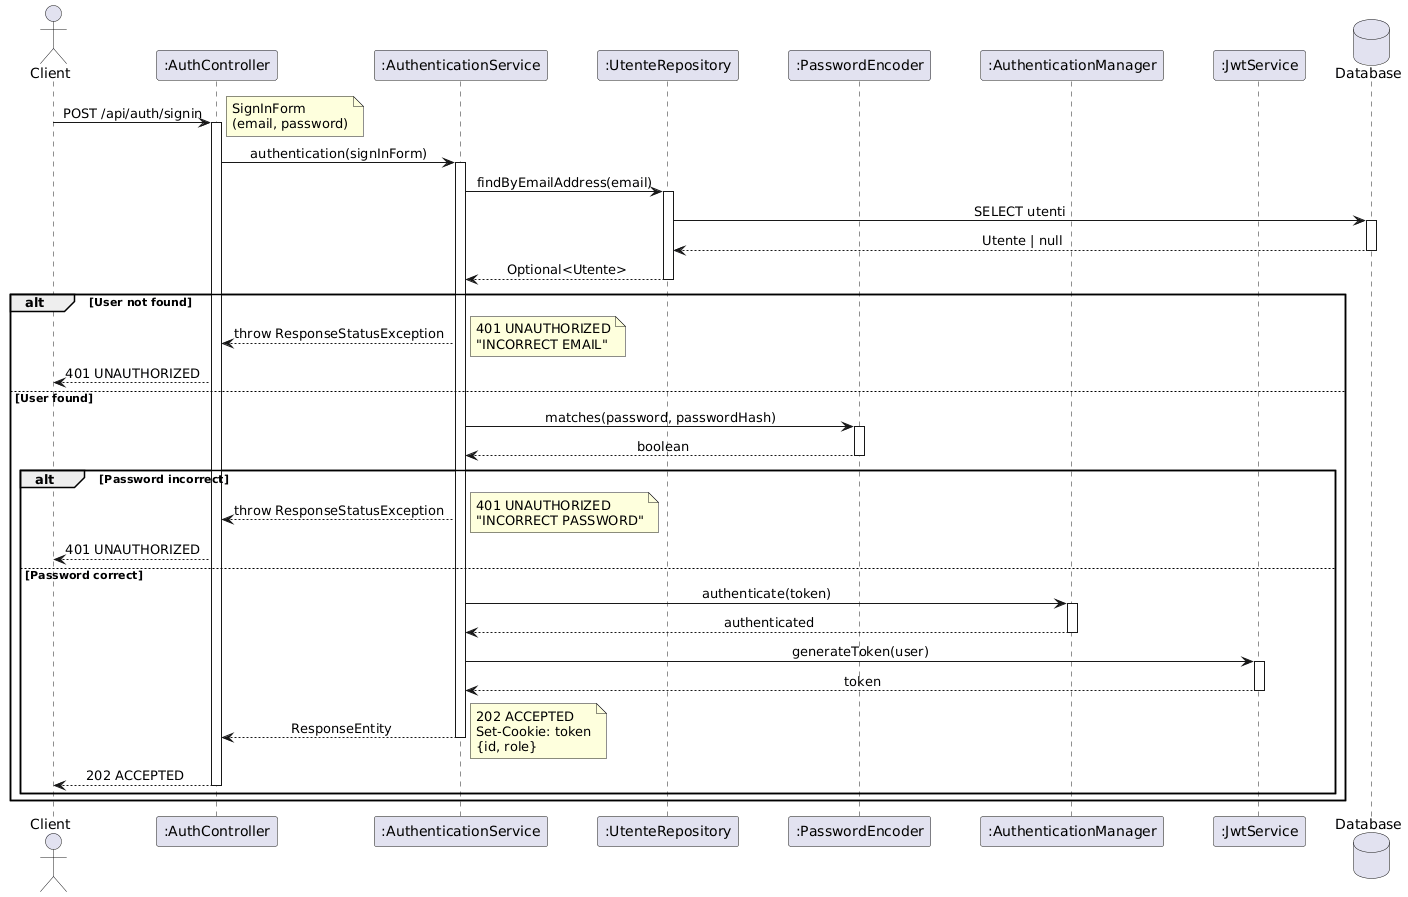
\includegraphics[width=\textwidth, keepaspectratio]
    {img/UML/sequence_authentication.png}
    \caption{Diagramma di sequenza UML - Autenticazione}
    \label{fig:seq_uml_authentication}
\end{figure}

\textbf{Flusso principale:}
\begin{enumerate}
    \item L'utente invia credenziali (email, password) via POST /api/auth/signin
    \item AuthController delega ad AuthenticationService
    \item Il sistema verifica l'esistenza dell'email tramite UtenteRepository
    \item PasswordEncoder valida la password tramite hash BCrypt
    \item AuthenticationManager autentica l'utente in Spring Security
    \item JwtService genera un token JWT firmato
    \item Il token viene inviato al client in un cookie HttpOnly sicuro
    \item Response 202 ACCEPTED con id utente e ruolo
\end{enumerate}

\textbf{Scenari alternativi:}
\begin{itemize}
    \item Email non esistente → 401 Unauthorized "INCORRECT EMAIL"
    \item Password errata → 401 Unauthorized "INCORRECT PASSWORD"
\end{itemize}
\newpage
\subsection{Registrazione utente}

La registrazione permette la creazione di nuovi account per pazienti, medici
o amministratori, con validazione univocità email e hash sicuro della password.

\begin{figure}[H]
    \centering
    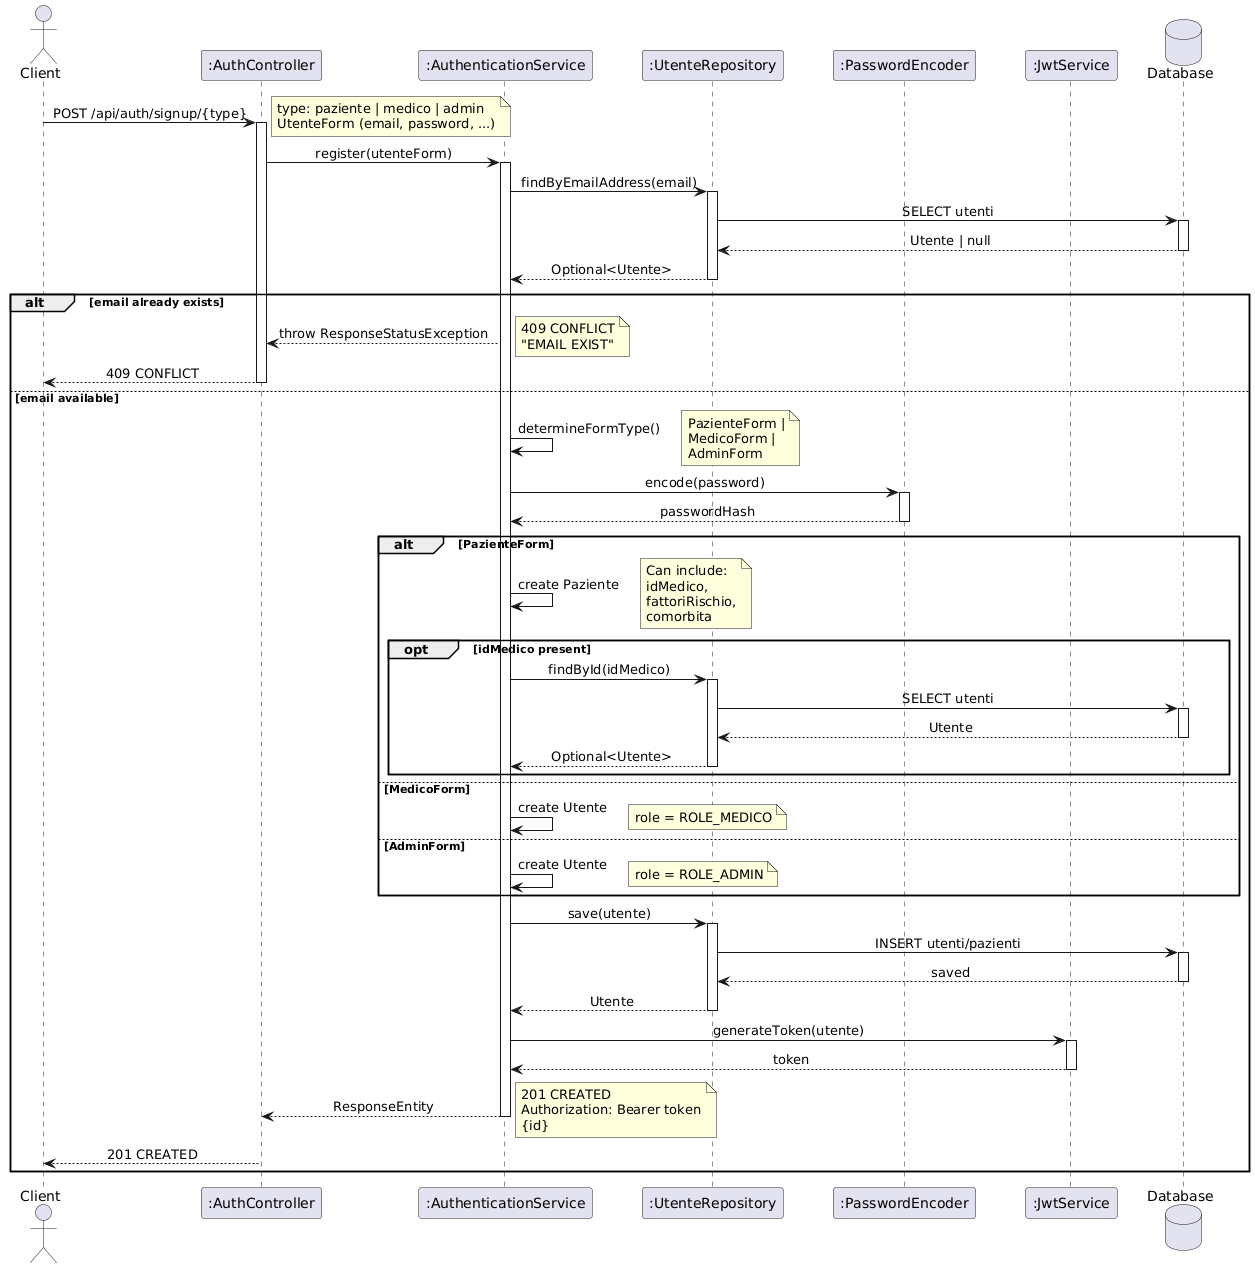
\includegraphics[width=\textwidth, keepaspectratio]
    {img/UML/sequence_registration.png}
    \caption{Diagramma di sequenza UML - Registrazione}
    \label{fig:seq_uml_registration}
\end{figure}
\newpage
\textbf{Caratteristiche:}
\begin{itemize}
    \item Endpoint differenziati: /api/auth/signup/\{paziente|medico|admin\}
    \item Verifica univocità email nel database
    \item Hash della password con BCrypt (PasswordEncoder)
    \item Tipologia utente determinata dal Form ricevuto
    \item Per i pazienti: possibilità di associare medico curante (idMedico opzionale)
    \item Generazione token JWT post-registrazione
    \item Response 201 CREATED con token in header Authorization
\end{itemize}

\textbf{Gestione errori:}
\begin{itemize}
    \item Email già esistente → 409 CONFLICT "EMAIL EXIST"
    \item Dati form invalidi → 400 BAD REQUEST con dettagli validazione
\end{itemize}

%..............................................................................
\subsection{Creazione terapia}

Il medico può prescrivere una terapia farmacologica a un paziente specificando
farmaco, dosaggio e frequenza di assunzione.

\begin{figure}[H]
    \centering
    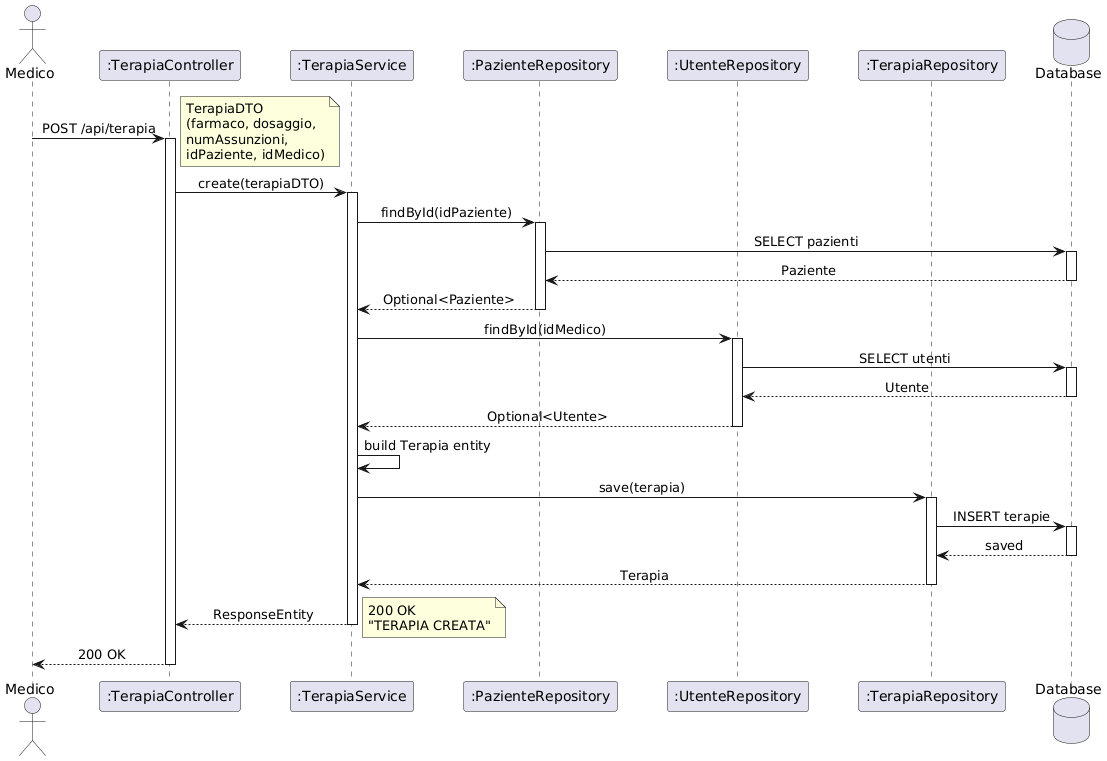
\includegraphics[width=0.9\textwidth, keepaspectratio]
    {img/UML/sequence_create_terapia.png}
    \caption{Diagramma di sequenza UML - Creazione terapia}
    \label{fig:seq_uml_create_terapia}
\end{figure}

\textbf{Dati della terapia (TerapiaDTO):}
\begin{itemize}
    \item \texttt{farmaco}: Nome del farmaco (String)
    \item \texttt{dosaggio}: Dosaggio prescritto (String, es. "500mg")
    \item \texttt{numAssunzioni}: Assunzioni giornaliere (Integer)
    \item \texttt{indicazioni}: Note terapeutiche opzionali (String)
    \item \texttt{idPaziente}: UUID del paziente
    \item \texttt{idMedico}: UUID del medico prescrittore
\end{itemize}

\textbf{Flusso:}
\begin{enumerate}
    \item Medico invia POST /api/terapia con TerapiaDTO
    \item TerapiaService recupera Paziente e Medico dai repository
    \item Crea entità Terapia con relazioni ManyToOne impostate
    \item Salva nel database tramite TerapiaRepository
    \item Response 200 OK "TERAPIA CREATA"
\end{enumerate}

%..............................................................................
\subsection{Inserimento rilevazione con alert automatico}

Quando il paziente inserisce una rilevazione glicemica, il sistema controlla
automaticamente se i valori sono fuori range normale e genera alert per il medico
in tempo reale.

\begin{figure}[H]
    \centering
    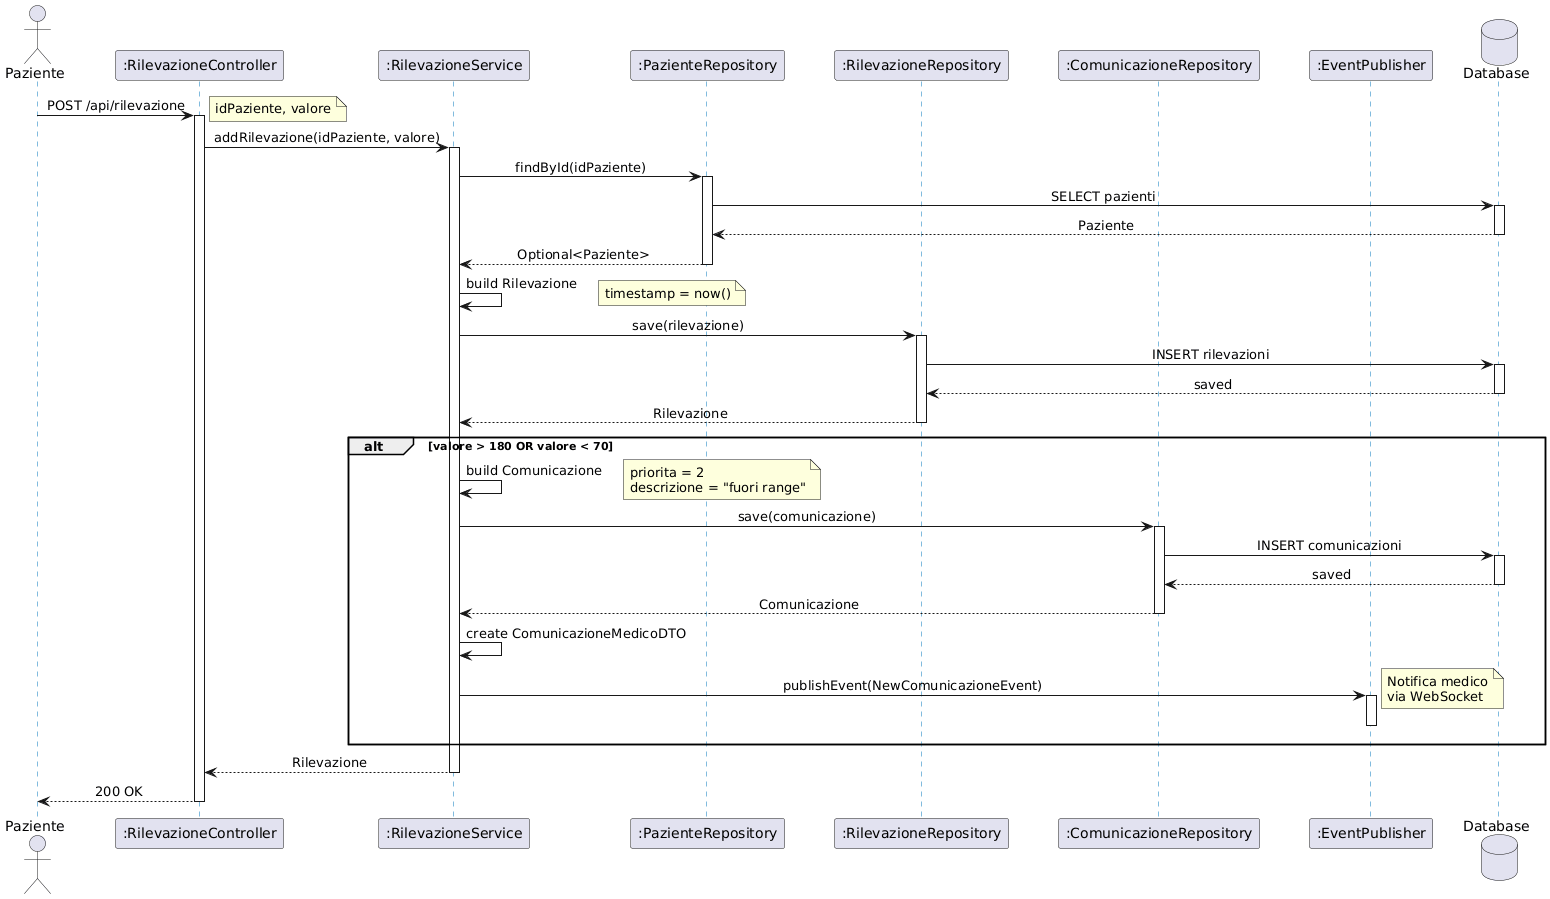
\includegraphics[width=0.9\textwidth, keepaspectratio]
    {img/UML/sequence_add_rilevazione.png}
    \caption{Diagramma di sequenza UML - Inserimento rilevazione}
    \label{fig:seq_uml_add_rilevazione}
\end{figure}

\textbf{Logica di alert automatico:}
\begin{itemize}
    \item Range glicemico normale: 80-130 mg/dL
    \item Condizione alert: valore < 80 OR valore > 130 OR valore > 180 (se dopo i pasti)
    \item Se fuori range:
    \begin{itemize}
        \item Crea Comunicazione con priorità 2 (media-alta)
        \item Descrizione: "Paziente ha inserito rilevazione fuori range (valore: X)"
        \item Salva comunicazione nel database
        \item Pubblica NewComunicazioneEvent via ApplicationEventPublisher
        \item Il medico riceve notifica real-time via WebSocket
    \end{itemize}
\end{itemize}

\textbf{Pattern utilizzati:}
\begin{itemize}
    \item Observer Pattern: pubblicazione evento per notifica asincrona
    \item Event-Driven Architecture: disaccoppiamento tra business logic e notifiche
\end{itemize}

%..............................................................................
\subsection{Filtro JWT per autenticazione richieste}

Ogni richiesta HTTP viene intercettata da JwtAuthenticationFilter che verifica 
la presenza e validità del token JWT, impostando il contesto di sicurezza Spring.

\begin{figure}[H]
    \centering
    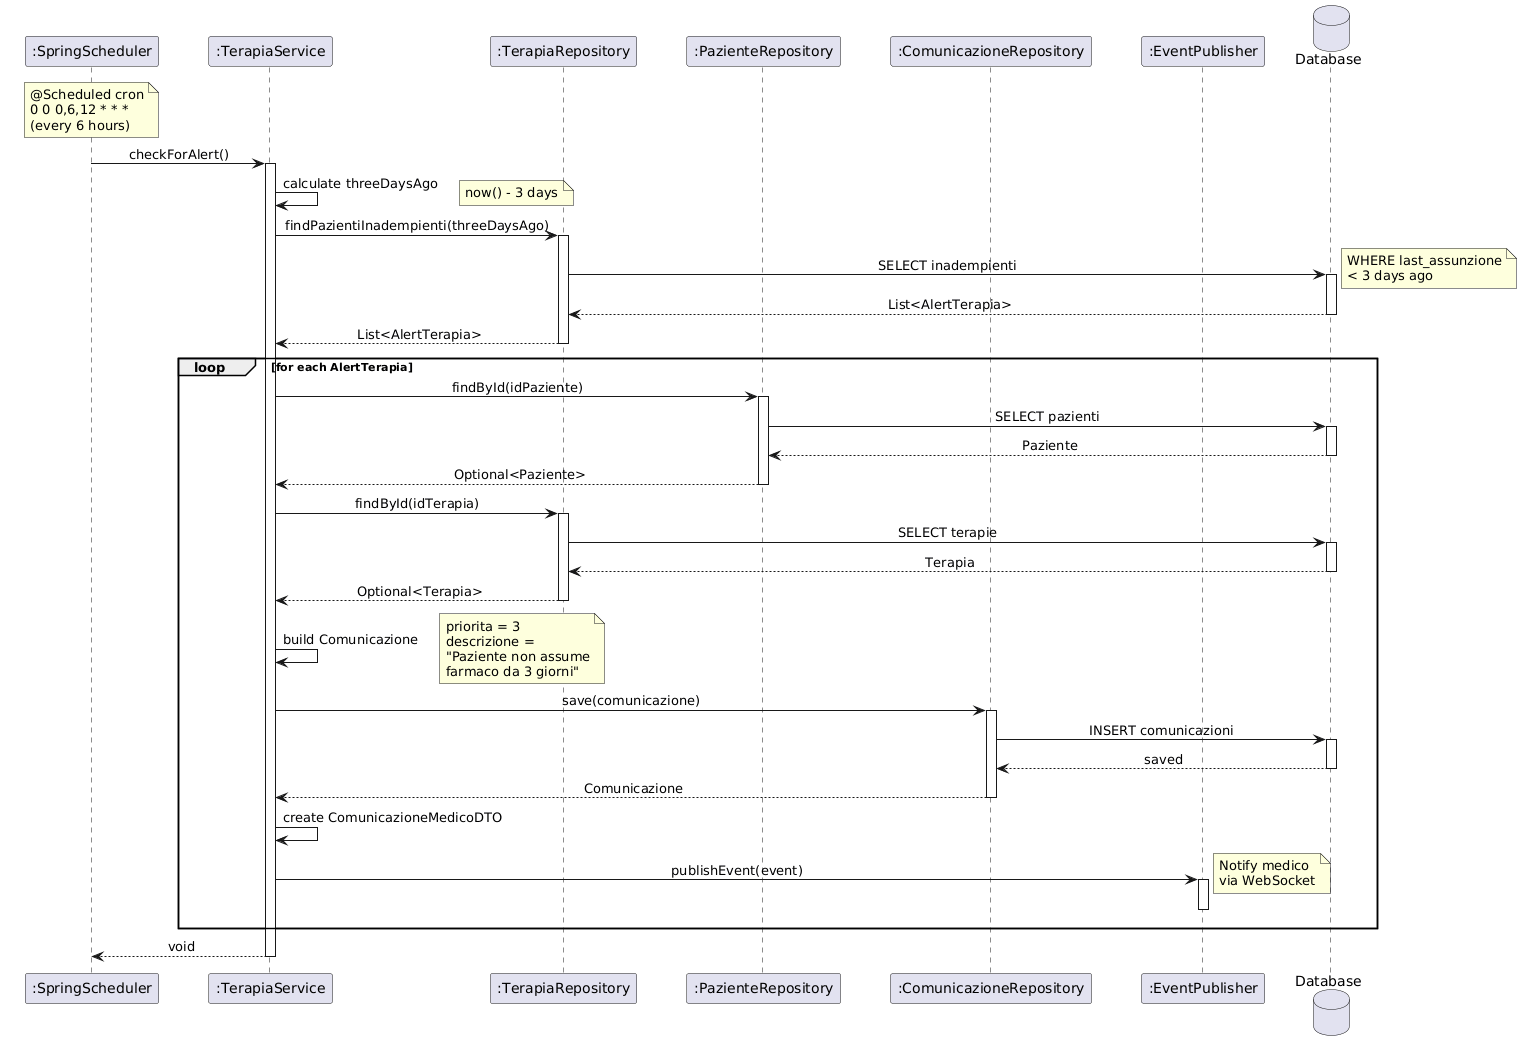
\includegraphics[width=0.9\textwidth, keepaspectratio]
    {img/UML/sequence_jwt_filter.png}
    \caption{Diagramma di sequenza UML - Filtro JWT}
    \label{fig:seq_uml_jwt_filter}
\end{figure}

\textbf{Processo di verifica token:}
\begin{enumerate}
    \item Filter intercetta richiesta HTTP (OncePerRequestFilter di Spring)
    \item Estrazione token dal cookie "token"
    \item JwtService verifica:
    \begin{itemize}
        \item Validità firma HMAC-SHA256
        \item Data scadenza (expiry claim)
        \item Assenza in blacklist (token non revocati)
    \end{itemize}
    \item Se valido:
    \begin{itemize}
        \item Estrae email dal claim "sub"
        \item Carica UserDetails dal database
        \item Crea UsernamePasswordAuthenticationToken
        \item Imposta SecurityContextHolder (contesto Spring Security)
    \end{itemize}
    \item Request procede nella FilterChain verso il Controller
    \item Controller può accedere a Principal autenticato
\end{enumerate}

\textbf{Gestione casi edge:}
\begin{itemize}
    \item Token assente: request procede senza autenticazione
    \item Token invalido/scaduto: request procede senza autenticazione
    \item Endpoint pubblici (/api/auth/**): nessuna autenticazione richiesta
\end{itemize}

%..............................................................................
\newpage
\subsection{Logout}

Il logout invalida il token JWT aggiungendolo a una blacklist persistente,
impedendo riutilizzo anche se non ancora scaduto.

\begin{figure}[H]
    \centering
    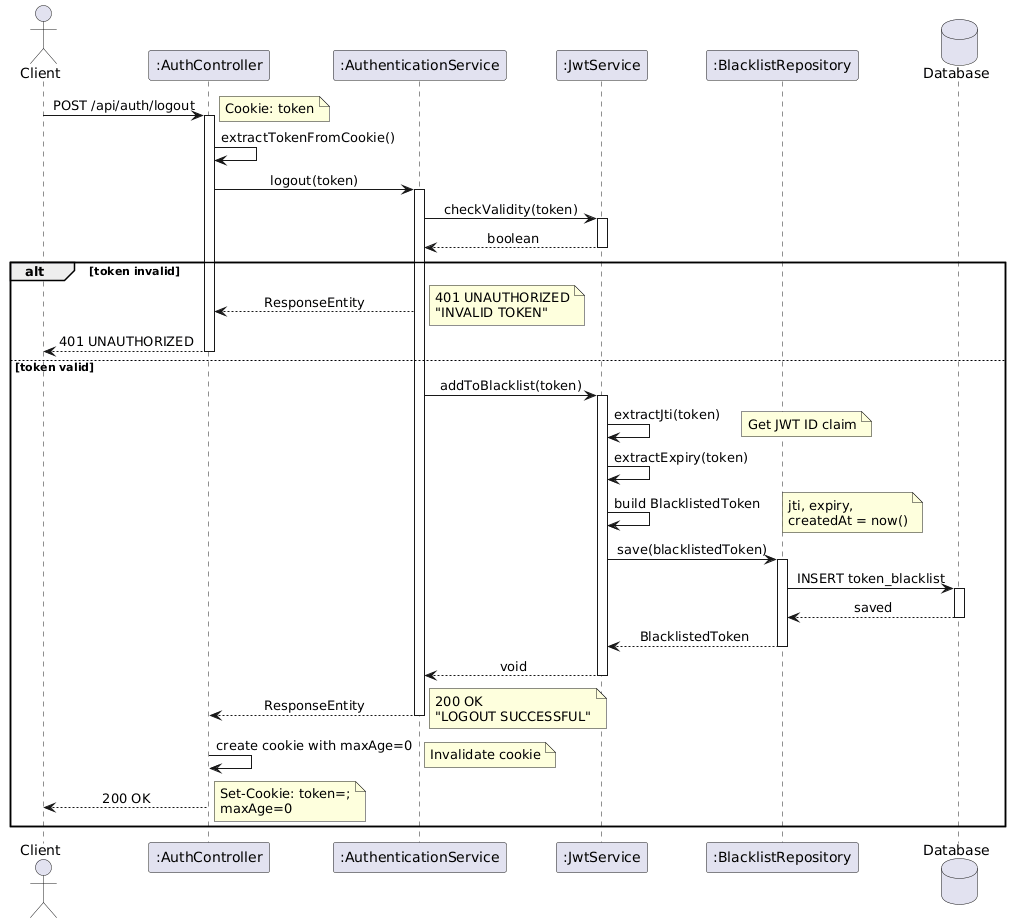
\includegraphics[width=\textwidth, keepaspectratio]
    {img/UML/sequence_logout.png}
    \caption{Diagramma di sequenza UML - Logout}
    \label{fig:seq_uml_logout}
\end{figure}

\textbf{Meccanismo blacklist:}
\begin{enumerate}
    \item Client invia POST /api/auth/logout con token in cookie
    \item AuthController estrae token dal cookie
    \item AuthenticationService verifica validità token
    \item JwtService:
    \begin{itemize}
        \item Estrae JWT ID univoco (claim "jti")
        \item Estrae data scadenza (claim "exp")
        \item Crea entità BlacklistedToken con (jti, expiry, createdAt=now())
        \item Salva in tabella token\_blacklist
    \end{itemize}
    \item AuthController crea cookie con maxAge=0 per invalidazione client-side
    \item Response 200 OK "LOGOUT SUCCESSFUL"
\end{enumerate}

\textbf{Cleanup automatico:}
\begin{itemize}
    \item La blacklist contiene solo token non ancora scaduti
    \item Task schedulato (opzionale) rimuove token scaduti periodicamente
    \item Verifica blacklist avviene ad ogni richiesta autenticata
\end{itemize}

%..............................................................................
\subsection{Controllo automatico terapie (Scheduled Task)}

Un task schedulato con annotazione @Scheduled controlla periodicamente i pazienti 
che non hanno assunto farmaci da almeno 3 giorni, generando alert per i medici.

\begin{figure}[H]
    \centering
    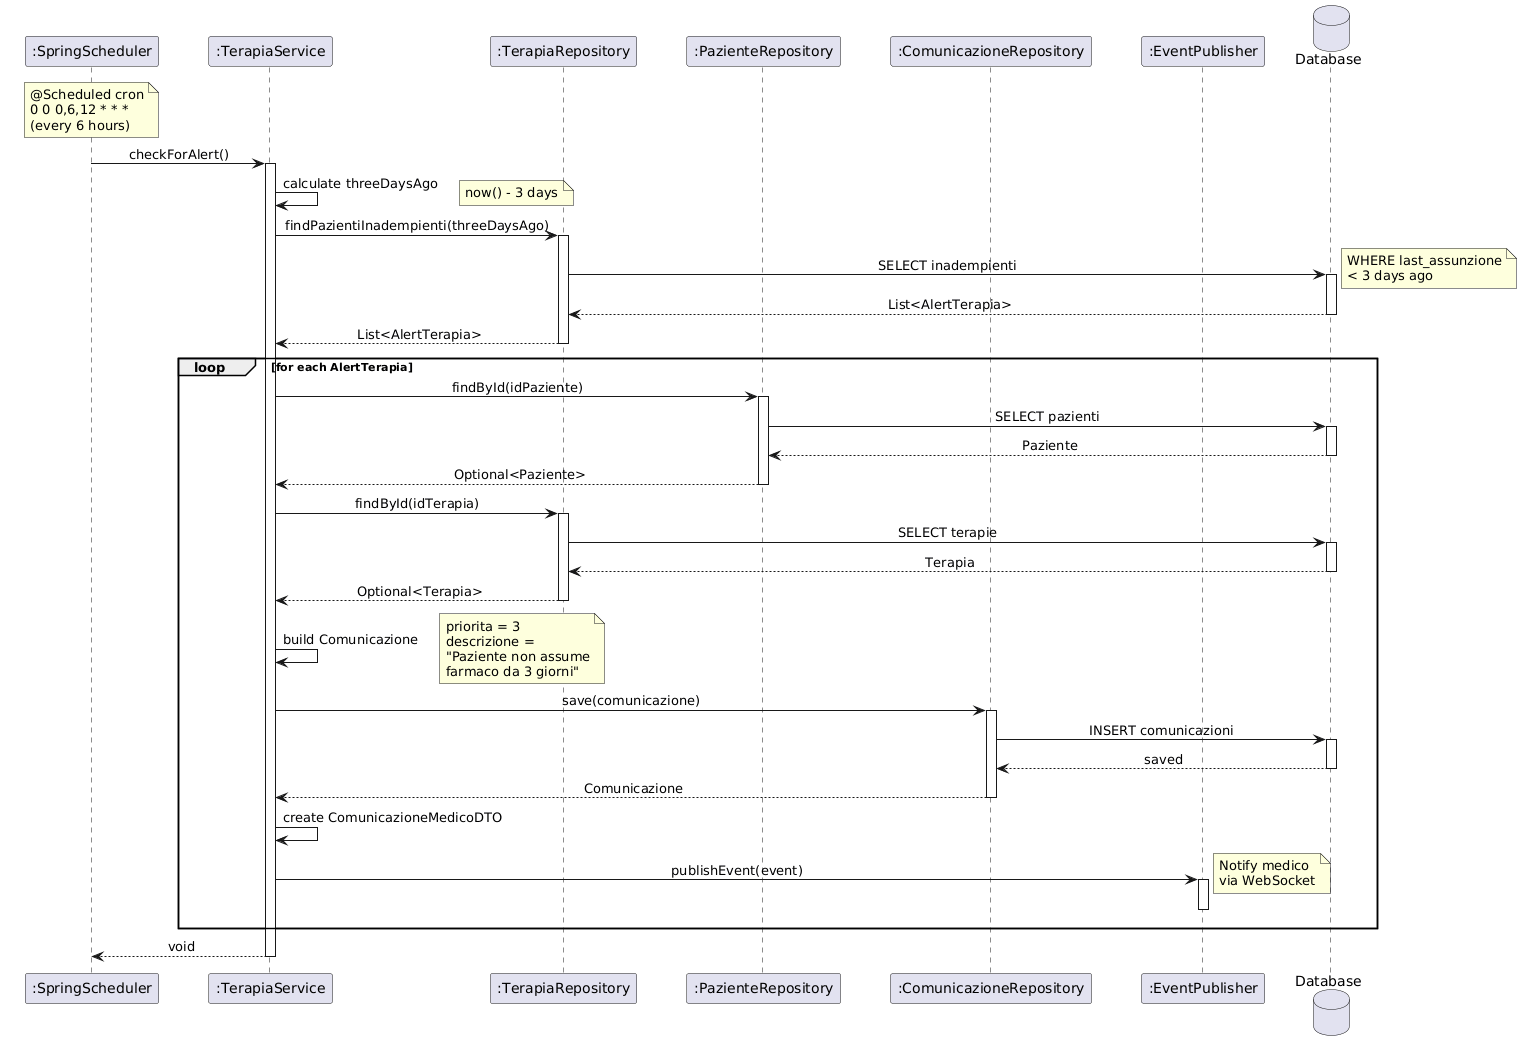
\includegraphics[width=0.9\textwidth, keepaspectratio]
    {img/UML/sequence_scheduled_therapy_check.png}
    \caption{Diagramma di sequenza UML - Controllo automatico terapie}
    \label{fig:seq_uml_scheduled_check}
\end{figure}

\textbf{Configurazione scheduling:}
\begin{itemize}
    \item Annotazione: \texttt{@Scheduled(cron = "0 0 0,6,12 * * *")}
    \item Esecuzione: ogni 6 ore (mezzanotte, 6:00, mezzogiorno)
    \item Timezone: Europe/Berlin
    \item Metodo: \texttt{TerapiaService.checkForAlert()}
\end{itemize}

\textbf{Logica di controllo:}
\begin{enumerate}
    \item Calcola threeDaysAgo = Instant.now() - Duration.ofDays(3)
    \item Query custom TerapiaRepository.findPazientiInadempienti(threeDaysAgo)
    \item Per ogni AlertTerapia trovato:
    \begin{itemize}
        \item Recupera Paziente e Terapia dai repository
        \item Crea Comunicazione con:
        \begin{itemize}
            \item priorita = 3 (alta)
            \item descrizione = "Paziente [nome] non assume [farmaco] da almeno 3 giorni"
            \item timestamp = now()
        \end{itemize}
        \item Salva comunicazione nel database
        \item Crea ComunicazioneMedicoDTO con dati paziente inclusi
        \item Pubblica NewComunicazioneEvent(idMedico, DTO)
        \item Medico riceve notifica real-time via WebSocket
    \end{itemize}
\end{enumerate}

\textbf{Query custom (JPQL):}
\begin{verbatim}
SELECT new AlertTerapia(t.id, p.id) 
FROM Terapia t 
JOIN t.idPaziente p 
LEFT JOIN Assunzione a ON a.idTerapia = t
WHERE a.timestamp IS NULL 
   OR a.timestamp < :threeDaysAgo
GROUP BY t.id, p.id
\end{verbatim}

\newpage

\chapter{Sviluppo del Software}
\section{Metodologia di sviluppo}
Per lo sviluppo del sistema è stato adottato un modello di processo iterativo e incrementale di matrice Agile, caratterizzato da un'elevata flessibilità operativa in funzione delle specificità progettuali. Il workflow, iniziato con l'analisi dei requisiti e la progettazione architetturale preliminare, si è articolato nella pianificazione ed esecuzione di Sprint focalizzati sull'implementazione. Al termine di ogni iterazione, si è proceduto sistematicamente alla validazione tramite test, all'aggiornamento della documentazione tecnica e alla revisione dei requisiti, garantendo così un miglioramento continuo del software. Per la gestione del codice è stata utilizzata una repository Github per 
facilitare la collaborazione tra i componenti del team grazie alla possibilità di lavorare su branch separati.
\begin{figure}[H]
    \centering
    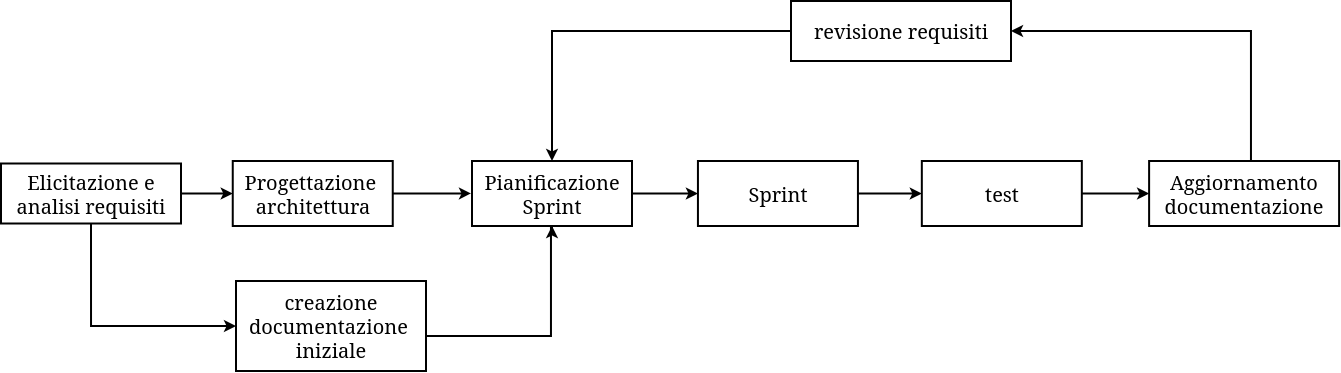
\includegraphics[width=\textwidth, height=\textheight, keepaspectratio]
    {img/Diagrammi/ProcessoSviluppo_tmp.png}
    \caption{Processo di sviluppo}
\end{figure}
\newpage
\section{Architettura}
Il software adotta un'architettura \textit{Client-Server} con elementi del pattern \textit{Model-View-Controller}.
Il sistema si compone di:

\begin{itemize}
  \item \textbf{Client (View)}: Interfaccia utente sviluppata in React 18 con TypeScript, responsabile della presentazione dati e dell'invio di richieste HTTP al server.
  
  \item \textbf{Server (Model + Controller)}: Implementato con Spring Boot (Java), suddiviso in:
    \begin{itemize}
      \item \textbf{Controller}: Gestisce le richieste della web API tramite Rest Controller, elaborandole attraverso il modello dati e restituendo risposte JSON.
      \item \textbf{Model}: Rappresenta i dati del sistema su H2 Database, gestendo la logica di business e le operazioni CRUD tramite Repository e Service.
    \end{itemize}
\end{itemize}

\begin{figure}[H]
    \centering
    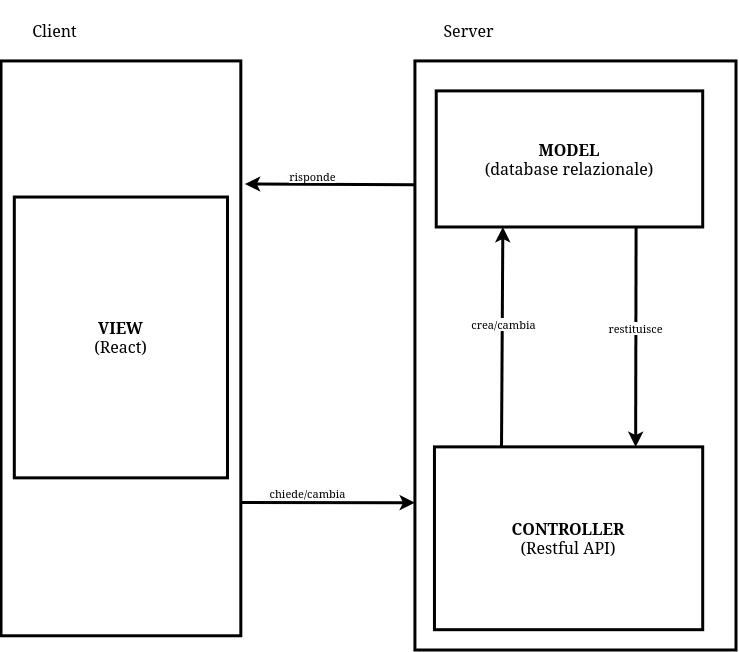
\includegraphics[width=0.7\textwidth, height=\textheight, keepaspectratio]
    {img/Diagrammi/architettura.png}
    \caption{Architettura del sistema}
\end{figure}

\subsection{Configurazione del Database}
Il sistema utilizza \textbf{H2 Database}, un database relazionale embedded in Java, configurato in modalità 
persistenza. La gestione avviene tramite console Web o chiamate API.

\subsubsection{Schema del Database}

Il database contiene le seguenti tabelle principali, generate automaticamente da JPA:

\begin{itemize}
    \item \texttt{utenti}: dati anagrafici e credenziali
    \item \texttt{pazienti}: estende utenti con dati specifici del paziente
    \item \texttt{rilevazioni}: valori glicemici registrati
    \item \texttt{terapie}: farmaci prescritti ai pazienti
    \item \texttt{assunzioni}: registrazioni delle assunzioni di farmaci
    \item \texttt{comunicazioni}: messaggi e alert tra paziente e medico
    \item \texttt{blacklisted\_tokens}: token JWT invalidati
    \item \texttt{logs}: tracciamento operazioni di sistema
\end{itemize}

Le relazioni principali collegano pazienti a medici (ManyToOne), rilevazioni/terapie/assunzioni ai rispettivi 
pazienti, e comunicazioni tra pazienti e medici.


\section{Pattern utilizzati}
Durante lo sviluppo del sistema sono stati implementati diversi design pattern, ciascuno scelto per risolvere 
specifiche problematiche architetturali e migliorare la manutenibilità del codice.

\subsection{Singleton}
Il Singleton, implemetato implicitamente attraverso l'uso dell'annotazione @Service del framework  è utilizzato per garantire che una classe servizio abbia una sola istanza e per fornire un unico punto di accesso globale a quell'istanza.

\subsection{Repository Pattern}
Implementato tramite Spring Data JPA, astrae l'accesso ai dati fornendo automaticamente metodi CRUD senza SQL 
manuale. Permette query personalizzate tramite metodi generati in utomatico dal framework Java Spring o JPQL, riducendo drasticamente il codice necessario.

\subsection{Observer Pattern}
Gestisce la comunicazione asincrona tramite il sistema di eventi di Spring. I Service pubblicano eventi 
significativi (es. rilevazioni anomale) che vengono intercettati da listener (es. WebSocket handler), garantendo 
disaccoppiamento tra logica di business e notifiche real-time.

\subsection{Facade Pattern}
I Service forniscono interfacce semplificate per operazioni complesse multi-sistema. Un esempio è il salvataggio 
di una rilevazione che orchestra automaticamente persistenza, verifica range, creazione alert, notifica WebSocket 
e logging.

\subsection{Builder Pattern}
Utilizzato per costruire oggetti complessi (entità JPA) in modo fluido tramite Lombok e \texttt{@Builder}, 
specificando solo i campi necessari ed evitando costruttori posizionali soggetti a errori.

\section{Implementazione}
\subsection{Struttura del Backend (Spring Boot)}
Il backend è organizzato seguendo una struttura modulare in package che favorisce 
la separazione delle responsabilità e la manutenibilità del codice:

\begin{itemize}
    \item \textbf{entity}: contiene le entità JPA che mappano le tabelle del database. 
    Ogni entità rappresenta un concetto del dominio applicativo (Utente, Paziente, 
    Rilevazione, Terapia, Comunicazione, Assunzione)
    
    \item \textbf{repository}: interfacce che estendono \texttt{JpaRepository} per 
    l'accesso ai dati. Spring Data JPA genera automaticamente l'implementazione dei 
    metodi CRUD e delle query personalizzate
    
    \item \textbf{service}: contiene la logica di business e orchestra le operazioni 
    tra repository e controller. I service gestiscono le transazioni e implementano 
    le regole applicative
    
    \item \textbf{controller}: espone le REST API tramite \texttt{@RestController}. 
    Ogni controller gestisce le richieste HTTP per una specifica area funzionale
    
    \item \textbf{dto}: Data Transfer Objects utilizzati per trasferire dati tra 
    client e server, separando la rappresentazione interna (entity) da quella esposta
    
    \item \textbf{config}: configurazioni del sistema (sicurezza, JWT, WebSocket, CORS)
    
    \item \textbf{filter}: filtri per l'elaborazione delle richieste HTTP, in particolare 
    il filtro JWT per l'autenticazione
    
    \item \textbf{forms}: classi per la validazione dei dati in ingresso dalle richieste
    
    \item \textbf{event}: gestione degli eventi applicativi per comunicazioni asincrone
    
    \item \textbf{exception}: gestione centralizzata delle eccezioni
\end{itemize}


\subsection{Repository Layer}

Il layer Repository utilizza Spring Data JPA per astrarre l'accesso al database.
Ogni repository estende \texttt{JpaRepository<Entity, UUID>} che fornisce automaticamente:

\begin{itemize}
    \item Metodi CRUD: \texttt{save()}, \texttt{findById()}, \texttt{findAll()}, 
    \texttt{deleteById()}
    \item Query personalizzate tramite naming convention dei metodi
    \item Paginazione e ordinamento
    \item Gestione transazionale automatica
\end{itemize}

\textbf{Repository implementati:}
\begin{itemize}
    \item \texttt{UtenteRepository}: gestione utenti con metodo 
    \texttt{findByEmailAddress(String email)}
    \item \texttt{PazienteRepository}: operazioni specifiche sui pazienti
    \item \texttt{RilevazioneRepository}: query sulle rilevazioni con metodi come 
    \texttt{findByIdPaziente\_Id(UUID)} e \texttt{findAllByPazienteIdMedicoId(UUID)}
    \item \texttt{TerapiaRepository}: gestione terapie
    \item \texttt{AssunzioneRepository}: registrazione assunzioni
    \item \texttt{ComunicazioneRepository}: gestione comunicazioni
    \item \texttt{BlacklistedTokenRepository}: gestione token JWT invalidati
\end{itemize}

Spring Data JPA genera automaticamente l'implementazione basandosi sul nome del metodo,
navigando le relazioni delle entità.

\subsection{Service Layer}
I Service orchestrano le operazioni tra Controller e Repository:
\begin{itemize}
    \item \textbf{UtenteService}: Operazioni CRUD su utenti con validazione.

    \item \textbf{PazienteService}: Gestione pazienti inclusa assegnazione medico e aggiornamento dati clinici.

    \item \textbf{RilevazioneService}: Inserimento rilevazioni con controllo automatico range glicemici (alert se valore < 80 mg/dL o > 130 mg/dL o > 130 mg/dL dopo i pasti ), creando comunicazioni automatiche con priorità alta e notifiche WebSocket.

    \item \textbf{TerapiaService}: Gestione completa terapie farmacologiche.

    \item \textbf{AssunzioneService}: Registrazione e storico assunzioni medicinali.

    \item \textbf{ComunicazioneService}: Messaggistica paziente-medico con gestione stati lettura.

    \item \textbf{AuthenticationService}: Gestisce registrazione (con form diversificati per ruolo, crittografia BCrypt, generazione JWT), autenticazione (verifica credenziali, generazione token, creazione cookie HTTP-only) e logout (invalidazione token via blacklist).

    \item \textbf{JwtService}: Gestione completa token JWT (generazione con claims email/ruolo/id, validazione firma e scadenza, verifica blacklist).

\end{itemize}


\subsection{Controller Layer}

I Controller espongono REST API mappando richieste HTTP ai Service tramite annotazioni \texttt{@GetMapping}, 
\texttt{@PostMapping}, \texttt{@PutMapping}, \texttt{@DeleteMapping}:
\\

\begin{itemize}
    \item \textbf{AuthController}: Endpoint per registrazione, login, logout e validazione token.

    \item \textbf{RilevazioneController}: Gestione rilevazioni con endpoint per inserimento, recupero 
    (anche come DTO), eliminazione e visualizzazione filtrata per ruolo (admin vede tutto, medico solo suoi 
    pazienti, paziente solo proprie).

    \item \textbf{PazienteController}: Operazioni su pazienti inclusa assegnazione medico.

    \item \textbf{TerapiaController, AssunzioneController, ComunicazioneController}: Gestione rispettive entità.

    \item \textbf{UtenteController}: Gestione utenti principalmente per admin.
\end{itemize}

\subsection{Autenticazione e Sicurezza}
Il sistema implementa autenticazione JWT tramite Spring Security con componenti:

\begin{itemize}
    \item \textbf{JwtAuthenticationFilter}: Filtro che intercetta ogni richiesta, estrae token JWT dal cookie, 
    valida tramite JwtService, carica dettagli utente e imposta autenticazione nel SecurityContext.

    \item \textbf{Token JWT}: Contiene header (algoritmo HS256), payload (subject email, claims id/ruolo, issued 
    at, expiration) e firma HMAC. La generazione avviene tramite metodo builder di Jwts, la validazione verifica 
    firma, scadenza e blacklist.

    \item \textbf{Flusso autenticazione}: Login valida credenziali con BCrypt, genera token JWT, crea cookie 
    HTTP-only; richieste successive includono cookie che viene validato dal filtro; logout aggiunge token a 
    blacklist.

    \item \textbf{Gestione ruoli}: ROLE\_ADMIN (accesso completo), ROLE\_MEDICO (gestione pazienti assegnati, 
    terapie, comunicazioni), ROLE\_PAZIENTE (solo dati personali). Controlli implementati nei Service con logica 
    condizionale basata su ruolo.

    \item \textbf{Sicurezza aggiuntiva}: Password con BCrypt mai in chiaro, campo \texttt{@JsonIgnore}; token 
    blacklist per logout sicuro; cookie HTTP-only contro XSS.

\end{itemize}

\subsection{Comunicazione Real-time con WebSocket}
Il sistema implementa WebSocket per notifiche real-time tramite due handler:

\begin{itemize}
    \item \textbf{ComunicazioneWebSocketHandler}: Gestisce connessioni persistenti medico-server usando mappa 
    concorrente delle sessioni. Ascolta eventi \texttt{NewComunicazioneEvent} e invia notifiche JSON immediate 
    al medico interessato.

    \item \textbf{LogsWebSocketHandler}: Fornisce streaming real-time dei log di sistema agli admin connessi per 
    monitoraggio operazioni e debugging.

    \item \textbf{Configurazione}: Classe config con \texttt{@EnableWebSocket} registra 
    handler su endpoint\\ \texttt{comunicazioni:?id=idMedico} e \texttt{/ws/logs}.

    \item \textbf{Flusso notifiche}: Rilevazione anomala → RilevazioneService crea Comunicazione → Pubblica 
    evento → Handler cattura e invia via WebSocket → Frontend mostra alert real-time. Sistema basato su eventi 
    garantisce disaccoppiamento tra logica business e notifiche.

\end{itemize}

\subsection{Data Transfer Objects (DTO)}

I DTO separano la rappresentazione interna (Entity) da quella esterna (API).

\textbf{DTO principali:}
\begin{itemize}
    \item \textbf{RilevazioneUtenteDTO}: rilevazione con dati utente inclusi
    \item \textbf{ComunicazioneMedicoDTO}: comunicazione con info paziente
    \item \textbf{PazienteForm}: validazione dati registrazione paziente
    \item \textbf{MedicoForm}: validazione registrazione medico
    \item \textbf{SignInForm}: validazione credenziali login
\end{itemize}

\textbf{Vantaggi dei DTO:}
\begin{itemize}
    \item Evitano esposizione di dati sensibili (es. password)
    \item Prevengono serializzazione ricorsiva di relazioni
    \item Permettono validazione specifica per operazione
    \item Riducono payload di rete (solo campi necessari)
    \item Disaccoppiano API da struttura database
\end{itemize}

\subsection{Gestione delle eccezioni}

Il sistema implementa gestione centralizzata degli errori.

\textbf{Meccanismi:}
\begin{itemize}
    \item \texttt{ResponseStatusException}: eccezioni con HTTP status
    \item Try-catch nei service con logging
    \item Propagazione eccezioni ai controller
    \item Risposta JSON strutturata per errori
\end{itemize}


\subsection{Logging}

Sistema di logging implementato con SLF4J e Logback.

\textbf{Livelli di log utilizzati:}
\begin{itemize}
    \item \texttt{INFO}: operazioni normali (login, registrazione, operazioni CRUD)
    \item \texttt{WARN}: situazioni anomale ma gestibili
    \item \texttt{ERROR}: errori che impediscono operazioni
\end{itemize}

\textbf{Esempi:}
\begin{verbatim}
logger.info("Tentativo di login per email: " + email);
logger.warn("Tentativo di login con email non esistente");
logger.error("Errore durante salvataggio: " + e.getMessage());
\end{verbatim}

\subsection{Struttura del Frontend (React + TypeScript)}

Il frontend è sviluppato con React 18 e TypeScript, organizzato per favorire 
riusabilità e manutenibilità.

\textbf{Struttura directory principale:}
\begin{itemize}
    \item \texttt{src/components/}: componenti React riutilizzabili
    \item \texttt{src/pages/}: pagine principali dell'applicazione
    \item \texttt{src/services/}: moduli per chiamate API
    \item \texttt{src/context/}: Context API per stato globale
    \item \texttt{src/hooks/}: custom hooks
    \item \texttt{src/types/}: definizioni TypeScript
    \item \texttt{src/utils/}: funzioni di utilità
\end{itemize}

\subsubsection{Gestione dello stato globale}

Utilizzo di React Context API per stato condiviso:

\textbf{AuthContext:}
\begin{itemize}
    \item Gestisce stato autenticazione
    \item Memorizza token JWT
    \item Fornisce funzioni login/logout
    \item Protegge route private
\end{itemize}

\textbf{UserContext:}
\begin{itemize}
    \item Memorizza dati utente loggato
    \item Fornisce info ruolo per rendering condizionale
    \item Gestisce aggiornamento profilo
\end{itemize}

\subsubsection{Comunicazione con il Backend}

Tutte le chiamate API sono gestite tramite Axios con configurazione centralizzata:

\textbf{Interceptor richieste:}
\begin{itemize}
    \item Aggiunge automaticamente credenziali (cookie con token)
    \item Imposta headers comuni
    \item Logging richieste in sviluppo
\end{itemize}

\textbf{Interceptor risposte:}
\begin{itemize}
    \item Gestione errori centralizzata
    \item Redirect a login se 401 Unauthorized
    \item Toast notification per errori
\end{itemize}

\subsubsection{Type Safety con TypeScript}

Definizione di interfacce per type safety completo:

\begin{verbatim}
interface Utente {
    id: string;
    email: string;
    nome: string;
    cognome: string;
    dataNascita: string;
    ruolo: 'ROLE_PAZIENTE' | 'ROLE_MEDICO' | 'ROLE_ADMIN';
}

interface Rilevazione {
    id: string;
    idPaziente: string;
    valore: number;
    timestamp: string;
}
\end{verbatim}

\subsubsection{Routing e navigazione}

React Router per navigazione SPA:

\begin{itemize}
    \item Route pubbliche: login, registrazione
    \item Route protette: dashboard, profilo, rilevazioni
    \item Guard basati su AuthContext
    \item Redirect automatico se non autenticati
\end{itemize}


\chapter{Test}
In questa fase del progetto ci siamo assicurati che tutte le funzionalità 
richieste fossero implementate e che i vari diagrammi fossero coerenti. \\
Successivamente abbiamo poi creato dei test automatizzati utilizzando JUnit
e Mockito con l'obbiettivo di verificare automaticamente il corretto
funzionamento di alcuni parti del codice. \\
Dopo l'esecuzione degli Unit test abbiamo svolto un test manuale dell'applicazione,
e infine, abbiamo fatto provare la webapp ad alcuni utenti esterni per ottenere un 
feedback da parte di un possibile utente della webapp.
\\
\section{Test automatici}
I nostri test automatici controllano il funzionamento dei service, ovvero
delle funzionalità dell'applicazione e delle possibilità offerte agli utenti.
\\ \\
In questi test come detto in precedenza abbiamo usato Mock per simulare repository
e dipendenze necessarie per testare automaticamente i seguenti service:
\begin{itemize}
    \item GlicemiawebApplicationTests.java : il test principale che verifica
    il corretto avvio del contesto di spring boot
    \item AssunzioneServiceTest.java : testa le funzionalità legate alle assunzioni
    di medicinali, cioè la possibilità del sistema di recuperare i dati necessari
    e la possibilità del paziente di registrarli
    \item AuthenticationServiceTest.java : viene testata l'autenticazione, sia
    per login che logout grazie all'utilizzo di un token JWT.
    \item ComunicazioneServiceTest.java : testa la comunicazione paziente-medico,
    si verifica la funzionalità di invio e ricezione dei messaggi e pure la possibilità
    del medico di segnare come letti i messaggi ricevuti
    \item PazienteServiceTest.java : testa delle funzionalità legate alla gestione
    del paziente, come la possibilità di recuperare i pazienti anche in base al medico,
    viene testata anche la possibilità di aggiornare i dati del paziente, l'associazione
    del medico e la gestione della password.
    \item RilevazioneServiceTest.java : testa l'inserimento e l'eliminazione di 
    una rilevazione da parte dell'utente, per la visualizzazione dei dati viene
    pure testata la possibilità di recuperarli ma con l'applicazione di filtri basati
    sul ruolo
    \item TerapiaService.java : testa la gestione delle terapie, quindi la creazione, modifica
    e l'eliminazione da parte del medico.
    \item UtenteServiceTest.java : testa la gestione di tutti gli utenti, quindi la creazione,
    la modifica e l'eliminazione di medici e pazienti.
\end{itemize}

\section{Test manuali}
Abbiamo poi eseguito dei test manuali per verificare il corretto funzionamento della applicazione, utilizzando
software come Postman o Insomnia per testare le API e tramite interfaccia grafica per della webapp seguendo l'utilizzo che ne farebbe un utente non sviluppatore.
di seguito le principali verifiche:
\begin{itemize}
    \item Verifica del corretto funzionamento dell'autenticazione
    \item Verifica del corretto funzionamento di tutte le funzionalità utente per utente
    \item Verifica di mancato salvataggio in caso di dati non validi o vuoti
\end{itemize}

\subsection{Test di un utente reale}
Infine abbiamo sottoposto degli utenti esterni alla nostra applicazione per avere un
un feedback da qualcuno di esterno che potrebbe essere un possibile utilizzatore
dell'applicazione.
In questa fase siamo stati solo osservatori e non abbiamo dato alcun tipo di informazione
su come utilizzare l'applicazione eccetto per le credenziali di accesso e lo scopo
della applicazione.
Grazie a questo test abbiamo migliorato l'applicazione in termini di user friendly
e a livello grafico.

\end{document}
